%%%%%%%%%%%%%%%%%%%%%%%%%%%%%%%%%%%%%%%%%%  不使用 authblk 包制作标题  %%%%%%%%%%%%%%%%%%%%%%%%%%%%%%%%%%%%%%%%%%%%%%
%-------------------------------PPT Title-------------------------------------
\title{第一原理计算软件简介与应用}
%-----------------------------------------------------------------------------

%----------------------------Author & Date------------------------------------
%\author[\textrm{Jun\_Jiang}]{姜\;\;骏\inst{}} %[]{} (optional, use only with lots of authors)
%% - Give the names in the same order as the appear in the paper.
%% - Use the \inst{?} command only if the authors have different
%%   affiliation.
\institute[BCC]{\inst{}%
%\institute[Gain~Strong]{\inst{}%
\vskip -20pt 北京市计算中心~云平台事业部~姜骏}
%\vskip -20pt {\large 格致斯创~科技}}
\date[\today] % (optional, should be abbreviation of conference name)
{	{\fontsize{6.2pt}{4.2pt}\selectfont{\textcolor{blue}{E-mail:~}\url{jiangjun@bcc.ac.cn}}}
\vskip 45 pt {\fontsize{8.2pt}{6.2pt}\selectfont{北京科技大学~理化楼-308% 报告地点
	\vskip 5 pt \textrm{2023.07.12}}}
}

%% - Either use conference name or its abbreviation
%% - Not really information to the audience, more for people (including
%%   yourself) who are reading the slides onlin%%   yourself) who are reading the slides onlin%%   yourself) who are reading the slides onlineee
%%%%%%%%%%%%%%%%%%%%%%%%%%%%%%%%%%%%%%%%%%%%%%%%%%%%%%%%%%%%%%%%%%%%%%%%%%%%%%%%%%%%%%%%%%%%%%%%%%%%%%%%%%%%%%%%%%%%%

\subject{}
% This is only inserted into the PDF information catalog. Can be left
% out.
%\maketitle
\frame
{
%	\frametitle{\fontsize{9.5pt}{5.2pt}\selectfont{\textcolor{orange}{“高通量并发式材料计算算法与软件”年度检查}}}
\titlepage
}
%-----------------------------------------------------------------------------

%------------------------------------------------------------------------------列出全文 outline ---------------------------------------------------------------------------------
\section*{}
\frame[allowframebreaks]
{
  \frametitle{Outline}
%  \frametitle{\textcolor{mycolor}{\secname}}
  \tableofcontents%[current,currentsection,currentsubsection]
}
%%在每个section之前列出全部Outline
%%类似的在每个subsection之前列出全部Outline是\AtBeginSubsection[]
%\AtBeginSection[]
%{
%  \frame<handout:0>%[allowframebreaks]
%  {
%    \frametitle{Outline}
%%全部Outline中,本部分加亮
%    \tableofcontents[current,currentsection]
%  }
%}

%-----------------------------------------------PPT main Body------------------------------------------------------------------------------------
\small
\frame
{
	\frametitle{材料计算软件发展现状}
\begin{figure}[h!]
\vspace*{-0.16in}
\centering
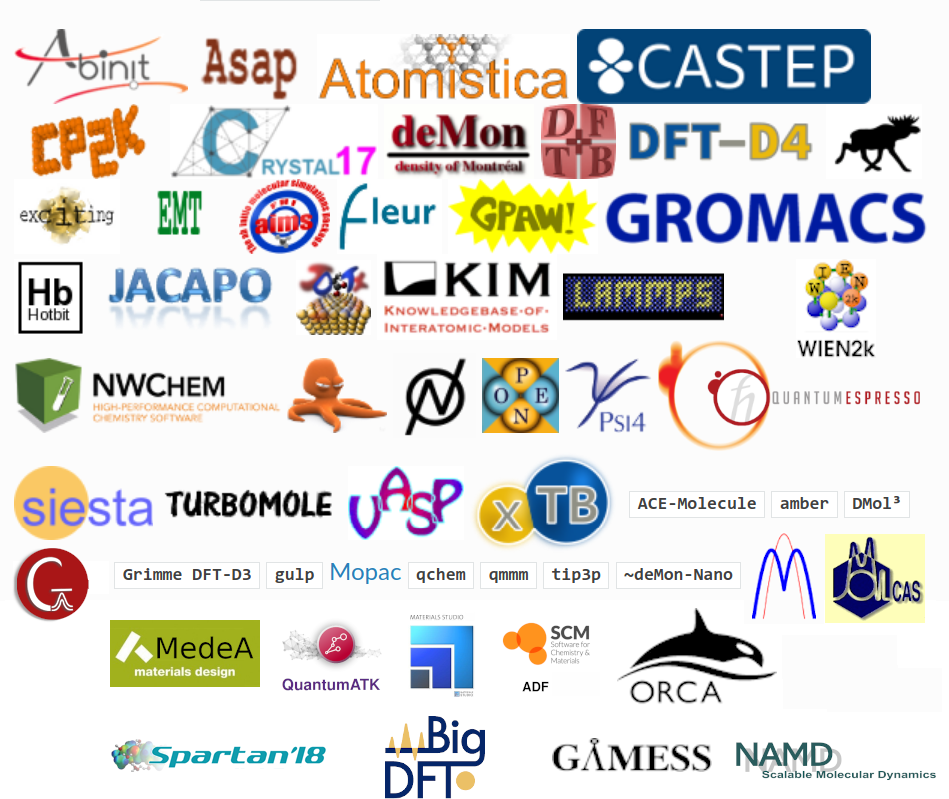
\includegraphics[width=3.30in]{Figures/Softwares_logo.png}
%\caption{\tiny \textrm{Pseudopotential for metallic sodium, based on the empty core model and screened by the Thomas-Fermi dielectric function.}}%(与文献\cite{EPJB33-47_2003}图1对比)
\label{Softwares}
\end{figure}
}

\frame
{
	\frametitle{国产第一原理计算软件现状}
\begin{figure}[h!]
\vspace*{-0.19in}
\centering
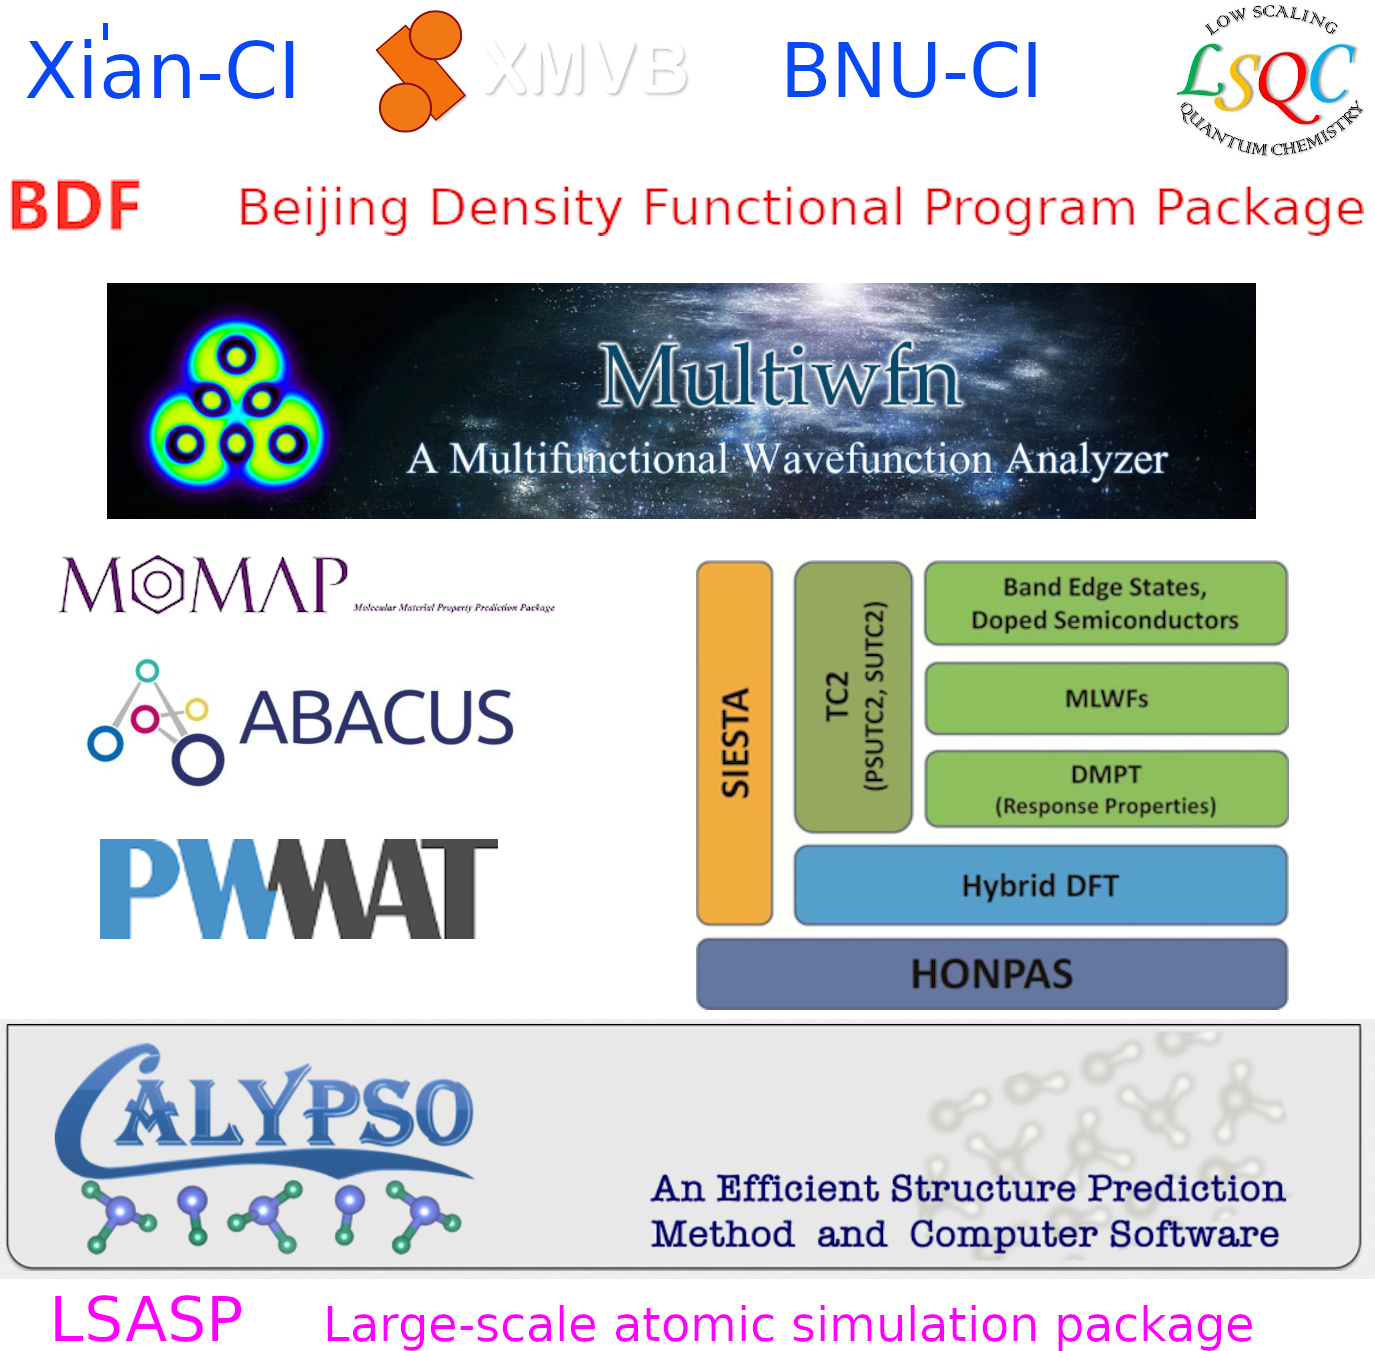
\includegraphics[width=2.83in]{Figures/Softwares_China-logo.png}
%\caption{\tiny \textrm{Pseudopotential for metallic sodium, based on the empty core model and screened by the Thomas-Fermi dielectric function.}}%(与文献\cite{EPJB33-47_2003}图1对比)
\label{Software-China}
\end{figure}
	\fontsize{6.2pt}{5.2pt}\selectfont{\textcolor{red}{中国学科发展战略\,$\cdot$\,理论与计算化学,~~国家自然科学基金委员会,~中国科学院,~~北京:~科学出版社,~~2016}}
}

\section{第一原理计算软件简介}
\frame
{
	\frametitle{\textrm{VASP}软件的特点}
	\textrm{VASP}软件是维也纳大学\textrm{(Universit\"at Wien)}~\textrm{G. Kresse}等开发的第一原理模拟软件包
	\begin{itemize}
		\item \textrm{VASP}采用\textrm{PAW~(Projector Augmented-Wave)}方法\upcite{VASP_manual},平衡了赝势方法和全电子计算优点,兼顾了计算的精度和效率
		\item \textrm{VASP}在实空间优化投影函数\textrm{(Projector)},将主要的计算过程变换到实空间完成,大大节省了内存的开销%,保证了计算精度和效率
		\item \textrm{VASP}通过引入多样的优化算法,提高了矩阵对角化和电荷密度搜索的效率
		\item 在\textrm{VASP}的并行计算中,有效均衡了各节点处理\textrm{FFT}变换负载和通信,提升了软件的并行效率
	\end{itemize}
	相比于其他第一原理计算软件,\textrm{VASP}从物理思想与方法、优化算法和并行计算实现等多个方面都有更为出色的性能
}

\frame
{
	\frametitle{\textrm{VASP}的开发团队}
\begin{figure}[h!]
\centering
\vspace*{-0.25in}
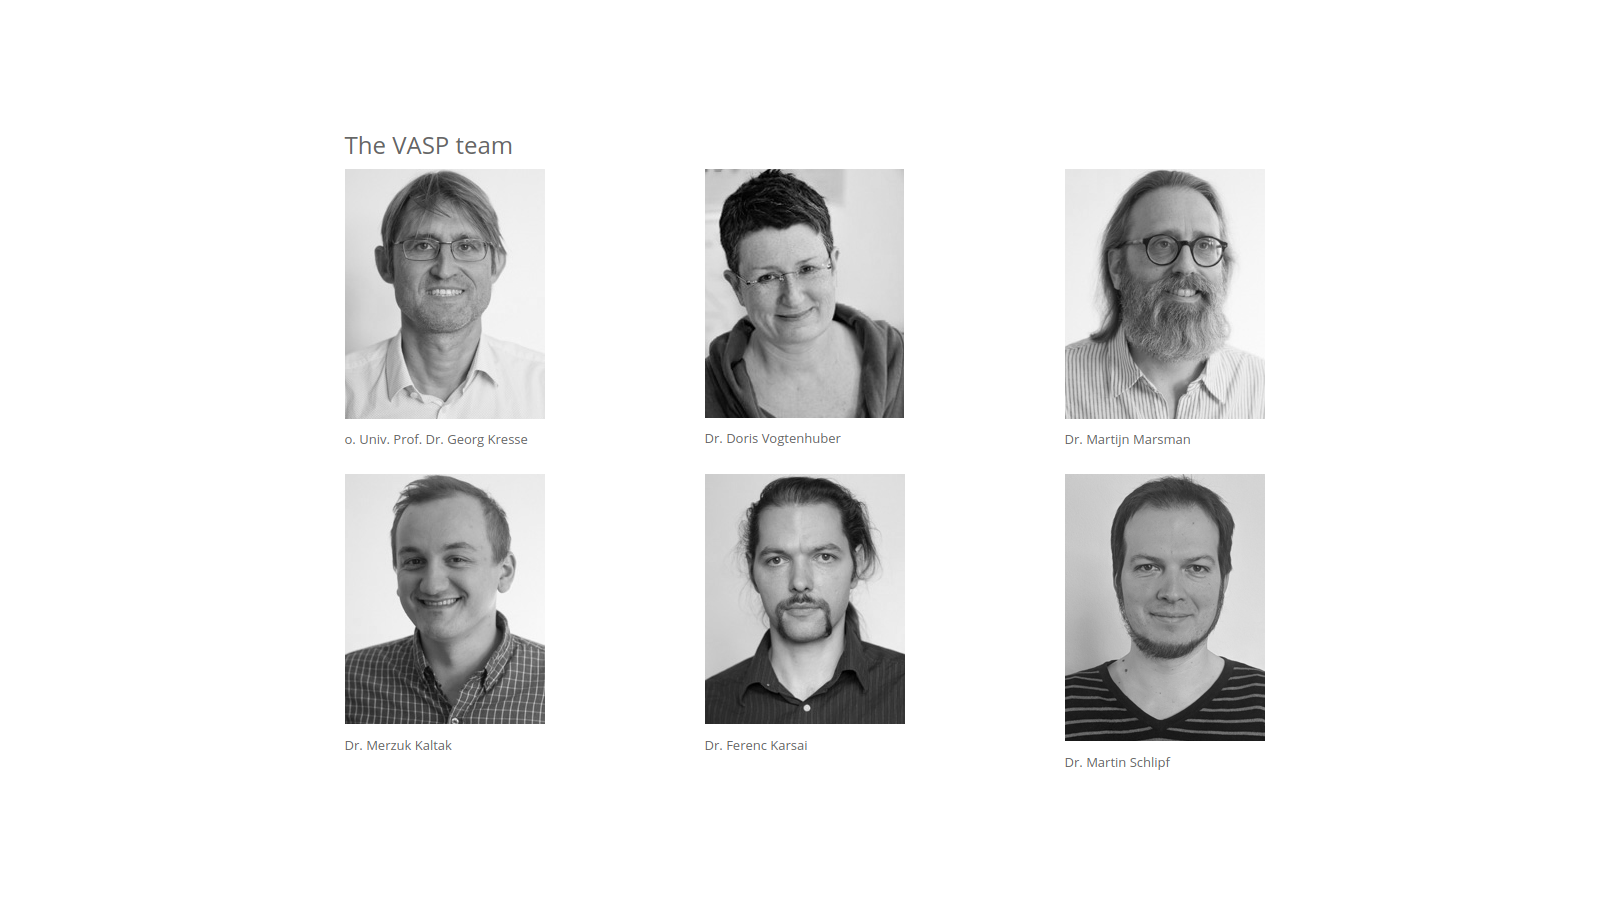
\includegraphics[height=2.70in,width=4.05in,viewport=330 130 1280 770,clip]{Figures/VASP_team.png}
\caption{\tiny \textrm{The development team of VASP.}}%(与文献\cite{EPJB33-47_2003}图1对比)
\label{VASP_team}
\end{figure}
}

\frame
{
	\frametitle{\textrm{VASP}的优化与迭代收敛}
	\textrm{VASP}计算中,资源消耗的主要部分是求解\textrm{Kohn-Sham}方程,即偏微分方程\textrm{(Partial Differential Equations,~PDE)}的自洽迭代, 迭代过程主要包括
	\begin{itemize}
		\item 矩阵的迭代对角化
		\item 电荷密度的自洽迭代
	\end{itemize}

	\vskip 10pt
	\textrm{VASP}的计算高效得益于求解过程中中应用了多种经典优化算法,保证了迭代计算的快速收敛
	\begin{itemize} 
		\item 拟牛顿法\textrm{(Quasi-Newton method)}
		\item 共轭梯度法\textrm{(Conjugate Gradients method, CG)}
		\item 残差最小化\textrm{(RMM-DIIS)}方法
	\end{itemize}
}

\frame
{
	\frametitle{\textrm{VASP}的\textrm{Kohn-Sham}方程求解流程}
\begin{figure}[h!]
	\vspace{-0.2in}
\centering
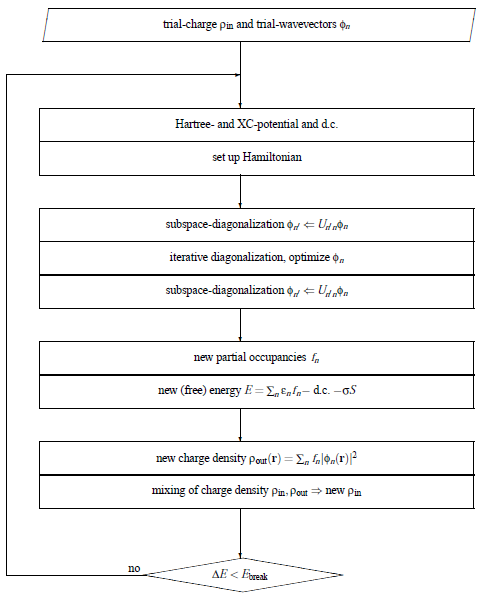
\includegraphics[height=2.75in,width=2.5in,viewport=0 0 480 630,clip]{Figures/VASP_procedure.png}
\caption{\tiny \textrm{The Flow of calculation for the KS-ground states.}}%(与文献\cite{EPJB33-47_2003}图1对比)
\label{PAW_baiseset}
\end{figure} 
}

\frame
{
	\frametitle{\textrm{VASP}的并行效率}
	与同类型软件相比,\textrm{VASP}有着优异的并行能力
\begin{figure}[h!]
	\vspace{-0.15in}
\centering
%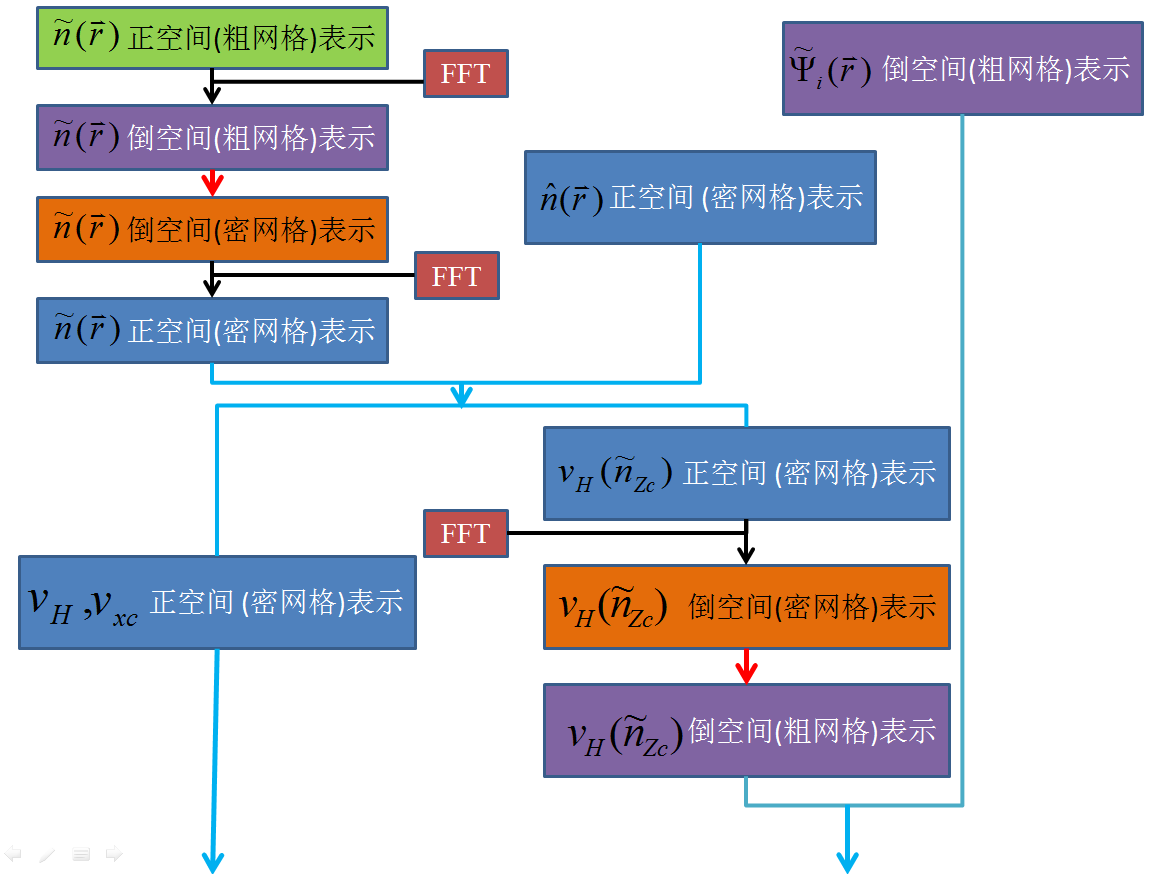
\includegraphics[height=2.7in,width=4.0in,viewport=0 0 1180 875,clip]{Figures/dual_grid.png}
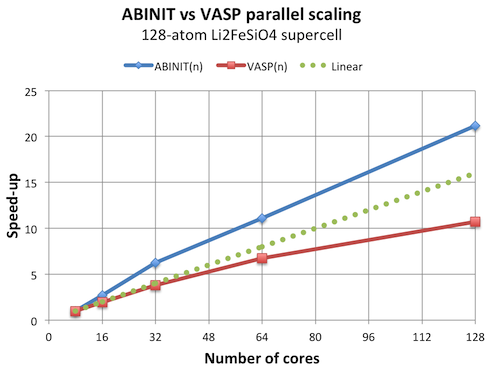
\includegraphics[height=1.55in,width=1.95in,viewport=0 0 240 200,clip]{Figures/VASP-abinit_Li128-1.png}
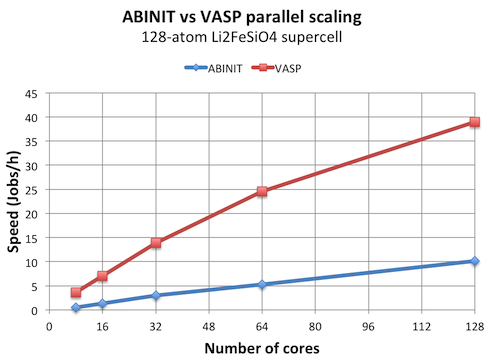
\includegraphics[height=1.55in,width=1.95in,viewport=0 0 240 200,clip]{Figures/VASP-abinit_Li128-2.png}
\caption{\tiny \textrm{The comparison of parallel scaling for ABINIT vs VASP.}}%(与文献\cite{EPJB33-47_2003}图1对比)
\label{ABINIT_vs_VASP}
\end{figure} 
\begin{itemize}
	\item \textrm{VASP}迭代对角化约束了矩阵的维度,减少了对角化过程中的迭代次数,保证了\textrm{MPI}并行的规模和扩展性
	\item \textrm{VASP}实施\textrm{FFT}变换时,保证各节点上处理的网格负载均衡
\end{itemize}
}

\frame
{
	\frametitle{\textrm{VASP}的通信开销}
	在高性能的计算队列中,\textrm{VASP}的并行上限可以突破256核,但当并行核数超过百核数量级,并行效率下降非常明显
\begin{figure}[h!]
	\vspace{-0.15in}
\centering
%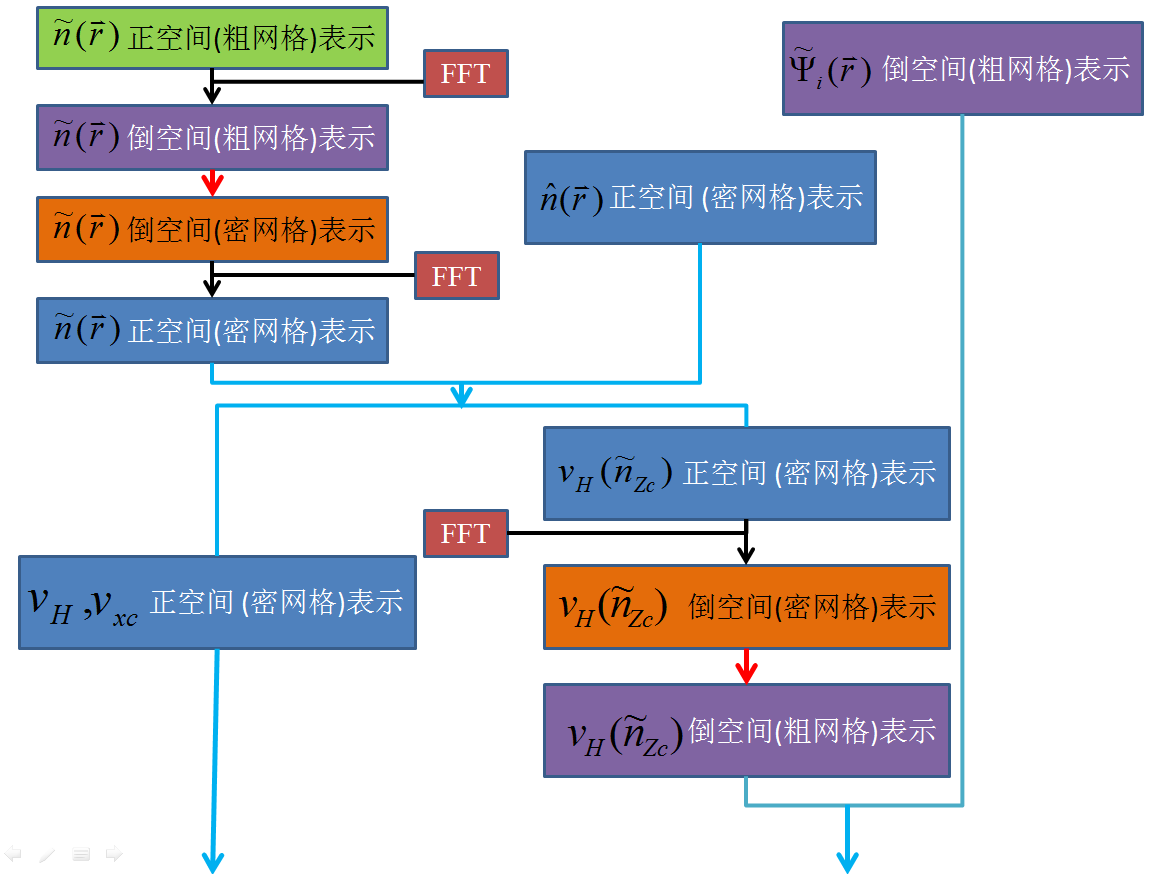
\includegraphics[height=2.7in,width=4.0in,viewport=0 0 1180 875,clip]{Figures/dual_grid.png}
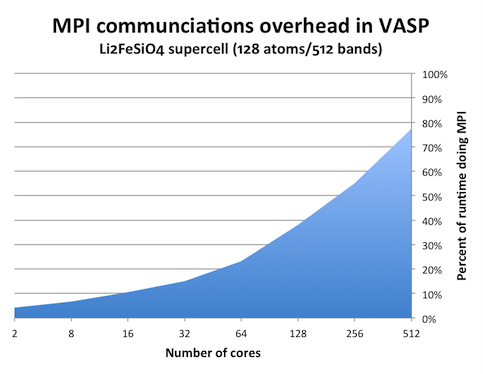
\includegraphics[height=1.55in,width=1.95in,viewport=0 0 240 200,clip]{Figures/VASP-mpi-Li128.png}
\caption{\tiny \textrm{Time spent in MPI calls with increasing the number of ranks in a VASP calculation.}}%(与文献\cite{EPJB33-47_2003}图1对比)
\label{VASP_communication}
\end{figure} 

如能对并行系统与\textrm{VASP}结合作深度改造(如国家超算天津中心方案),\textrm{VASP}的并行扩展可以到$10^4$核级别,但这一改造需要对底层代码和计算框架作较大规模改动
}

\frame
{
	\frametitle{\textrm{VASP}的\textrm{GPU}加速}
\textrm{NVIDIA}多年来致力于\textrm{VASP}的\textrm{GPU}加速,取得了一定的成效
\begin{figure}[h!]
	\vspace{-0.15in}
\centering
%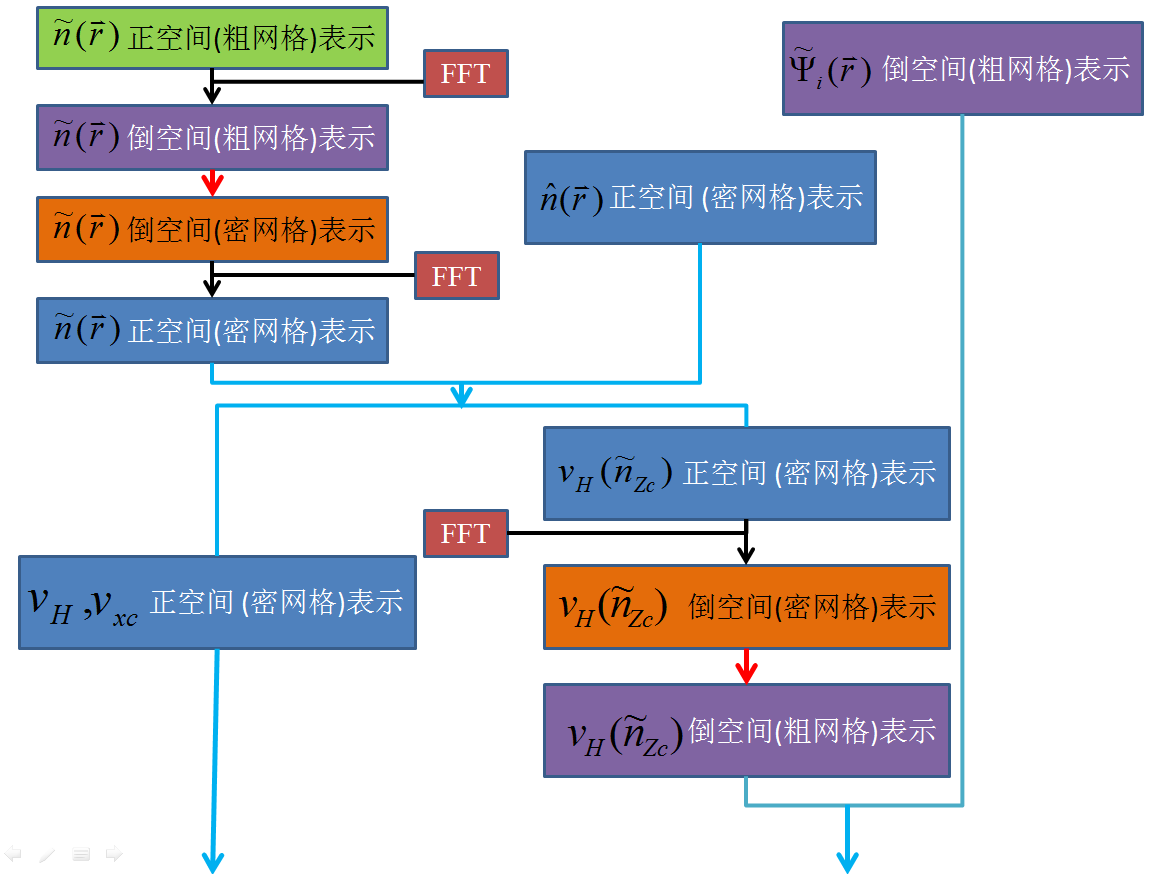
\includegraphics[height=2.7in,width=4.0in,viewport=0 0 1180 875,clip]{Figures/dual_grid.png}
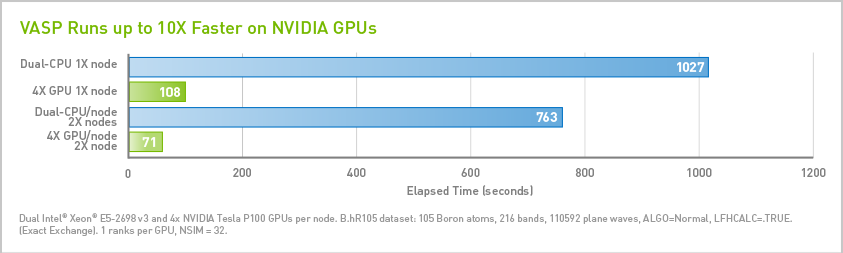
\includegraphics[height=1.2in,width=4.05in,viewport=0 0 850 260,clip]{Figures/VASP-GPU-CPU.png}
\caption{\tiny \textrm{Compare of VASP calculation with GPU and CPU.}}%(与文献\cite{EPJB33-47_2003}图1对比)
\label{VASP_GPU}
\end{figure} 
\begin{itemize}
	\item 通用配置下,\textrm{GPU}对\textrm{VASP}计算有加速效果,一般可提升4$\sim$6倍
	\item 矩阵对角化的并行算法限制了\textrm{GPU}在第一原理计算中的应用
	\item \textrm{GPU}加速的模式主要适合于分子动力学计算
\end{itemize}
}

\frame
{
	\frametitle{\textrm{VASP}软件概要}
	作为第一性原理计算的商用软件,\textrm{VASP}已成为计算材料学领域应用最广泛的软件之一。全球绝大多数超算中心都安装了\textrm{VASP},据统计,\textrm{VASP}软件的作业机时占用全球总机时的12$\sim$20\%,但由于其%类似于linpack软件,
属于重型浮点计算密集型应用,实际耗电量占比则高达30$\sim$50\%
\vskip 3pt
	{\fontsize{9.0pt}{7.2pt}\selectfont{
	\begin{itemize}
		\item \textcolor{blue}{物理上},\textrm{VASP}基于\textrm{DFT}近似,求解\textrm{Kohn-Sham}方程,并将粒子基态密度问题转化为矩阵的本征函数和本征值问题
		\item \textcolor{blue}{数学上},方程求解过程的核心是矩阵对角化与\textrm{PDE}的自洽迭代,即便对于简单体系,也需要完成数十次的迭代,而规模大的计算模拟体系则可能需要成千上万次迭代计算
		\item \textcolor{blue}{计算过程上},\textrm{VASP}计算的时长开销主要是本征值求解的矩阵对角化;此外由于算法限制,\textrm{Kohn-Sham}方程作为线性方程组作并行处理时,节点间存在密集的通信。在上千节点,上万计算核的大规模并行系统上,数据通信将严重影响程序的性能,这是当前\textrm{VASP}软件的主要瓶颈
	\end{itemize}}}
%			\textcolor{magenta}{有必要探索新的并行和优化策略来提升\textrm{VASP}的计算性能}
}

\frame
{
	\frametitle{\textrm{WIEN2k}软件简介}
\begin{figure}[h!]
\centering
\vspace*{-0.16in}
%\subfigure[\footnotesize{Logo of WIEN2k}]{
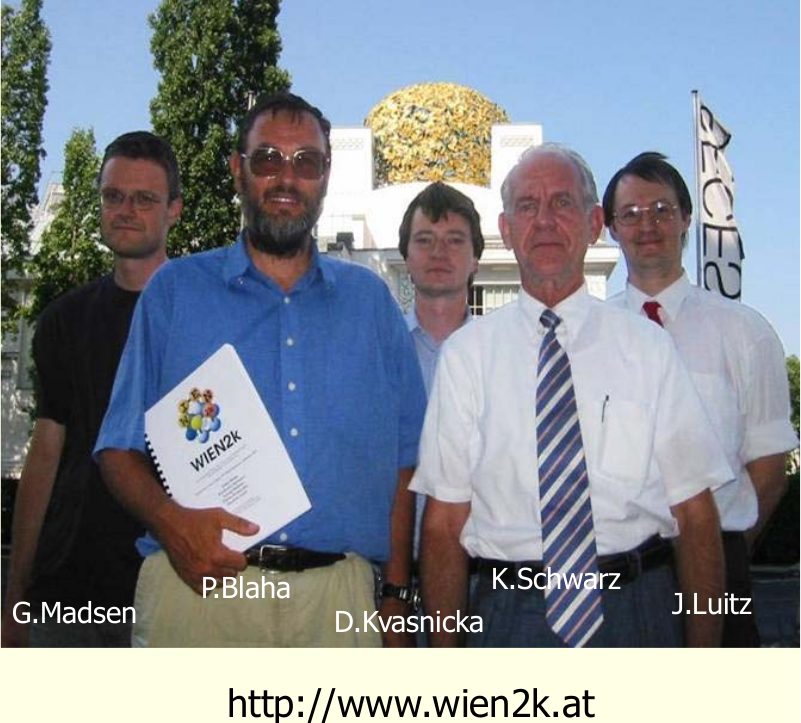
\includegraphics[height=1.5in]{Figures/WIEN2k-Group.png}
\hskip 0.5pt
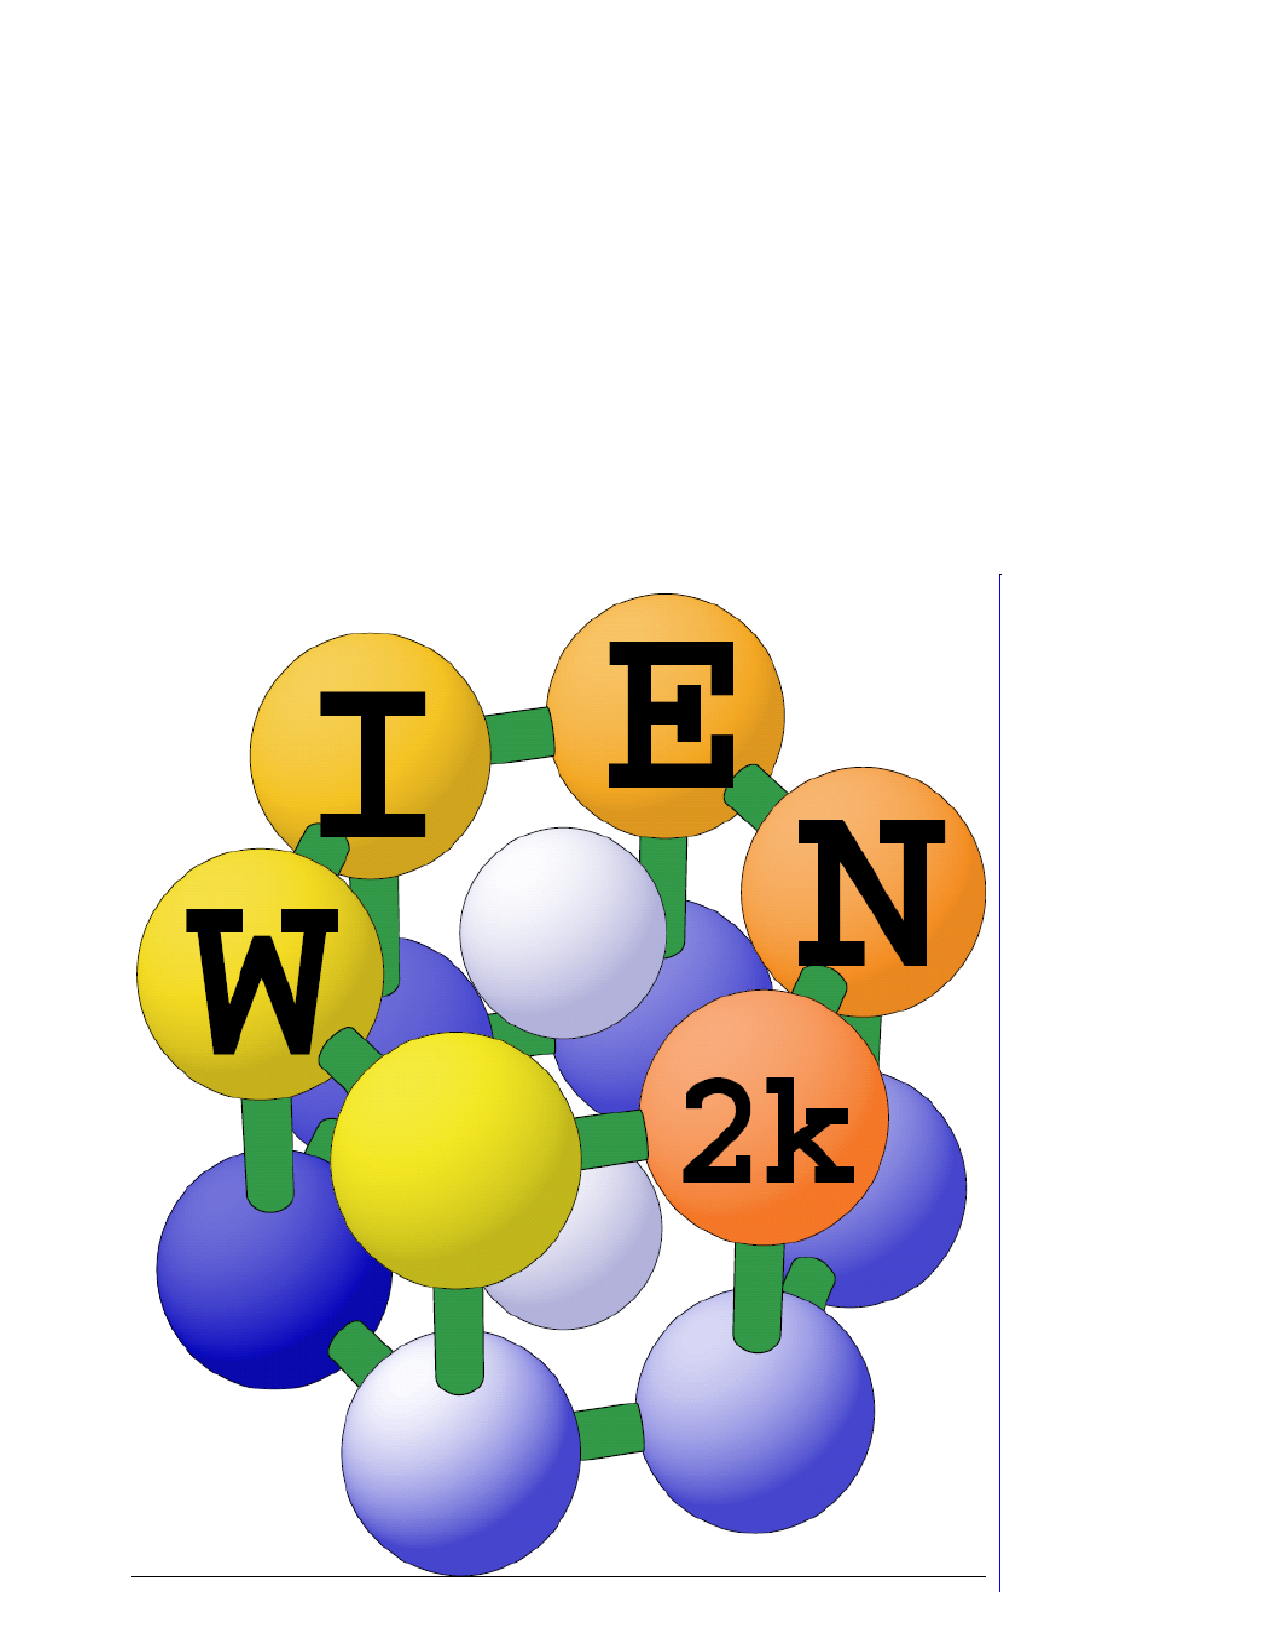
\includegraphics[height=1.5in,width=1.6in,viewport=13 35 475 515,clip]{Figures/logo_WIEN2k.pdf}
%\caption{\small \textrm{}}%(与文献\cite{EPJB33-47_2003}图1对比)
%\label{Brillouin_Cube}
%}
%\subfigure[\footnotesize{Logo of VASP}]{
%\includegraphics[height=1.48in,width=2.24in,viewport=55 145 595 455,clip]{logo_VASP.eps}
%\caption{\small \textrm{}}%(与文献\cite{EPJB33-47_2003}图1对比)
\label{Logo_of_WIEN2k}
%}
\end{figure}
\textrm{WIEN2k}是由奥地利维也纳技术大学\textrm{(Vienna University of Technology)}开发的高精度第一原理材料计算软件包\upcite{WIEN2k_UG}。%\\\textrm{WIEN2k};\textrm{VASP}。
\begin{itemize}
	\item 采用普适的全势\textrm{(Full-Potential, FP)}方法\\对计算对象的化学环境依赖小
	\item \textrm{LAPW}基组\\兼备描述波函数邻近原子核和位于原子核间行为的能力
	\item 计算精度高,结果常作为理论计算的\textrm{Benchmark}
%	\item \textrm{VASP}:采用\textrm{USPP-PAW}方法,计算效率高,特别擅长计算材料的力学性质\upcite{VASP_UG}
\end{itemize}
}

\frame
{
	\frametitle{\textrm{WIEN2k}软件简介}
\begin{minipage}[t]{0.55\textwidth}
	制约\textrm{WIEN2k}软件应用的主要因素
	\begin{itemize}
		\item 高精度计算必须付出的代价\\
			\textcolor{blue}{计算速度慢,处理体系有限}
		\item 各计算模块部分独立\\
			\textcolor{red}{输入控制文件过多}\\
			\textcolor{red}{输出数据文件分散}
		\item 采用\textrm{tcsh}脚本串联各部分\\
			计算中间结果需写入外部存储\\
			\textcolor{red}{\textrm{I/O}耗时过多}
		\item 软件的并行环境设置拙劣\\
			\textcolor{red}{\textrm{mpi}并行效率低下}
		\item \textcolor{red}{编译安装繁琐}
	\end{itemize}
\end{minipage}
\hfill
\begin{minipage}[t]{0.43\textwidth}
\begin{figure}[h!]
\centering
\vspace*{-10pt}
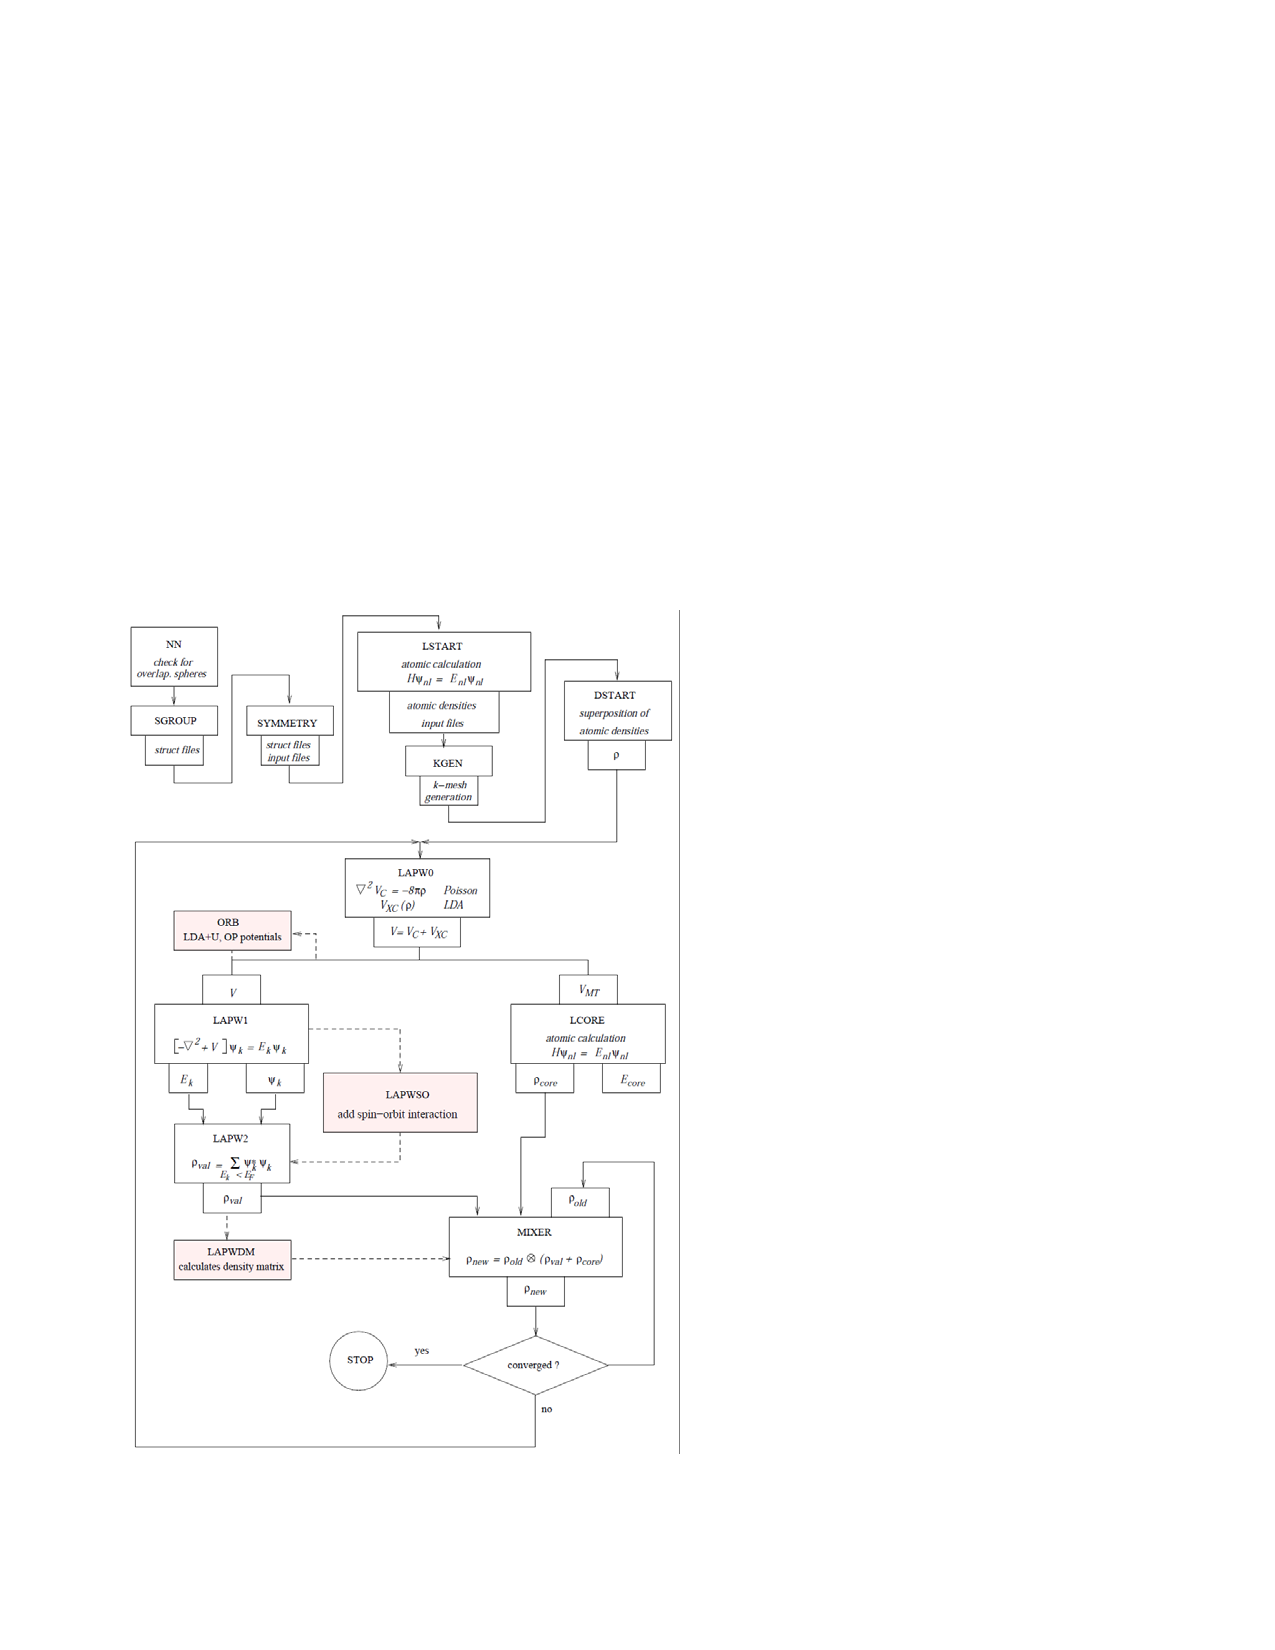
\includegraphics[height=2.6in,width=1.60in,viewport=60 90 325 500,clip]{Figures/WIEN2k_Program_flow.pdf}
\caption{\tiny \textrm{Program flow in WIEN2k.}}%(与文献\cite{EPJB33-47_2003}图1对比)
\label{WIEN2k_program_flow}
\end{figure}
\end{minipage}
}

\section{\rm{VASP}算例与\rm{WIEN2k}算例}
\frame
{
	\frametitle{\textrm{VASP}计算示范:~\textrm{Si}}
\vspace*{-13pt}
\begin{figure}[h!]
\centering
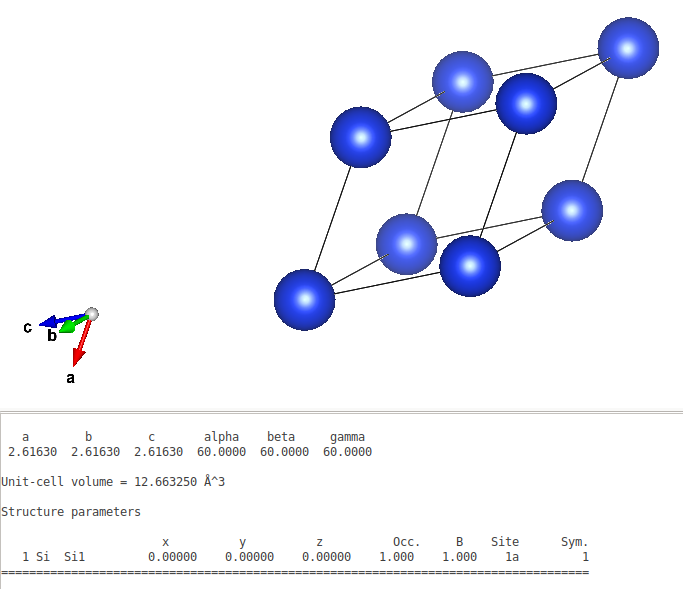
\includegraphics[height=1.78in]{Figures/VASP_example-Si_POSCAR-1-Fig.png}
\vskip 1pt
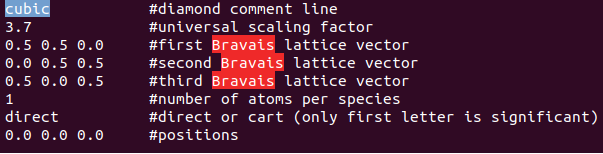
\includegraphics[height=0.98in]{Figures/VASP_example-Si_POSCAR-1.png}
%\caption{\tiny \textrm{The structure of TiC.}}%(与文献\cite{EPJB33-47_2003}图1对比)
\label{Fig:VASP-Si_POSCAR}
\end{figure}
}

\frame
{
	\frametitle{\textrm{VASP}计算示范:~\textrm{Si}}
\vspace*{-5pt}
\begin{figure}[h!]
\centering
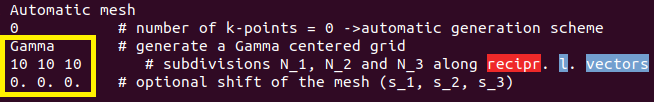
\includegraphics[height=0.62in]{Figures/VASP_example-Si_KPOINTS-G.png}
\vskip 4pt
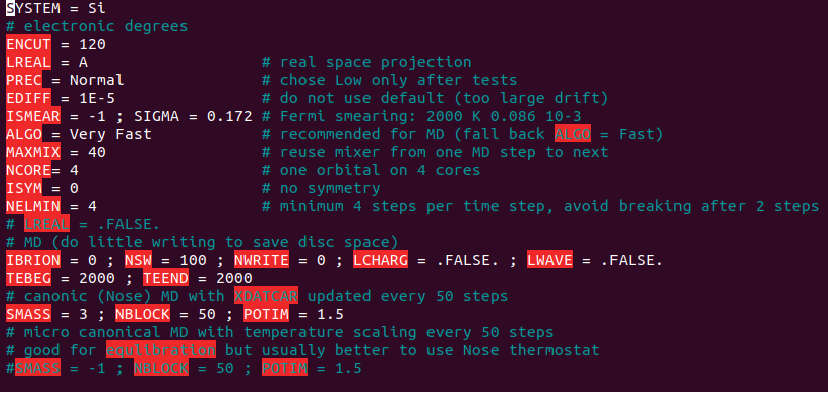
\includegraphics[height=1.88in]{Figures/VASP_example-Si_INCAR-dyn.png}
%\caption{\tiny \textrm{The structure of TiC.}}%(与文献\cite{EPJB33-47_2003}图1对比)
\label{Fig:VASP-Si_KPOINT-INCAR}
\end{figure}
}

\frame
{
	\frametitle{\textrm{VASP}计算示范:~\textrm{Si}}
\vspace*{-13pt}
\begin{figure}[h!]
\centering
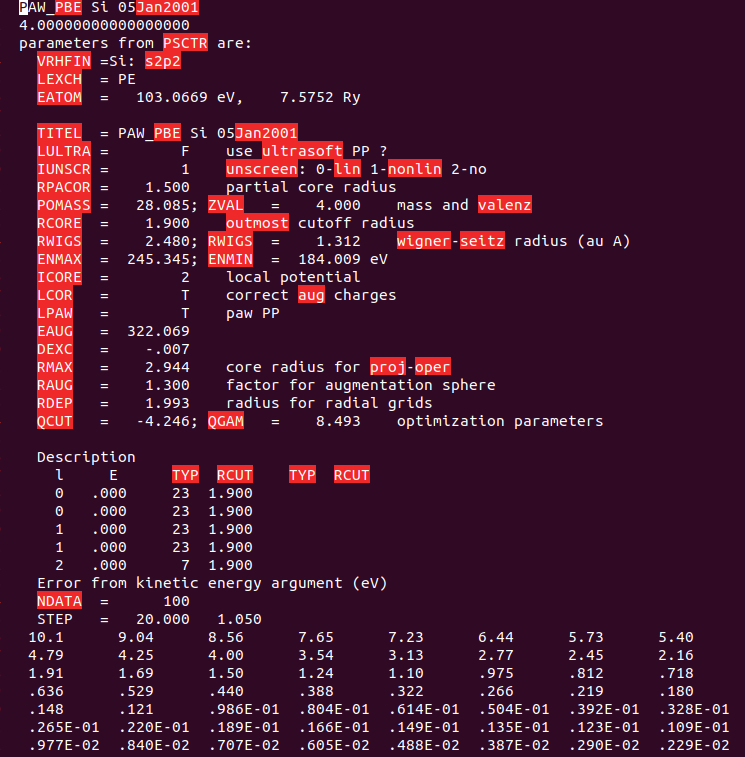
\includegraphics[height=2.88in]{Figures/VASP_example-Si_POTCAR.png}
%\caption{\tiny \textrm{The structure of TiC.}}%(与文献\cite{EPJB33-47_2003}图1对比)
\label{Fig:VASP-Si_POTCAR}
\end{figure}
}

\frame
{
	\frametitle{\textrm{VASP}计算示范:~\textrm{Si}}
\vspace*{-10pt}
\begin{figure}[h!]
\centering
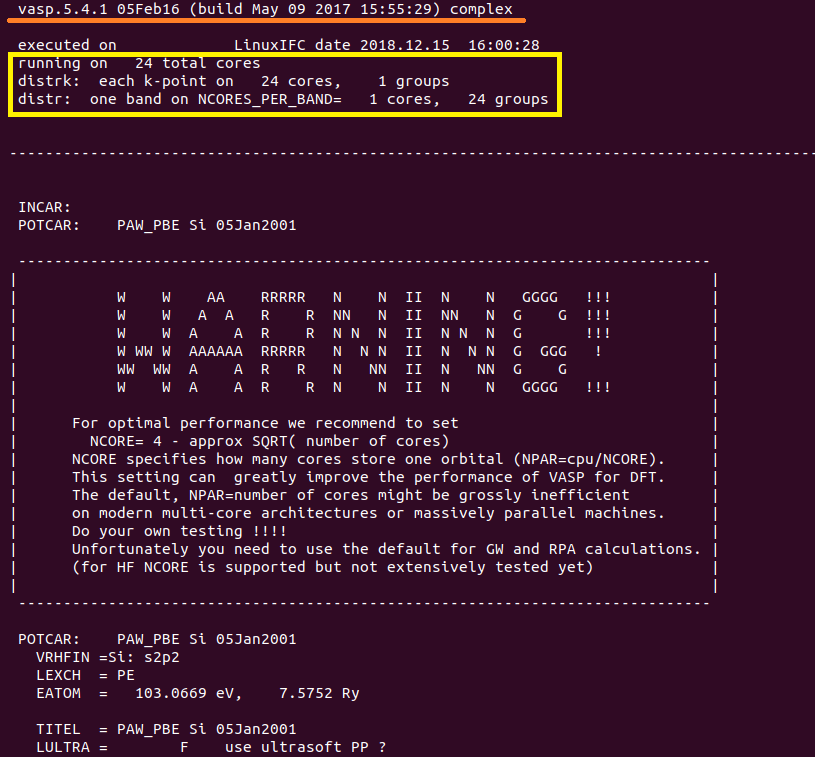
\includegraphics[width=3.0in]{Figures/VASP_example-Si_OUTCAR-1.png}
%\caption{\tiny \textrm{The structure of TiC.}}%(与文献\cite{EPJB33-47_2003}图1对比)
\label{Fig:VASP-Si_OUTCAR-part1}
\end{figure}
}

\frame
{
	\frametitle{\textrm{VASP}计算示范:~\textrm{Si}}
\vspace*{-10pt}
\begin{figure}[h!]
\centering
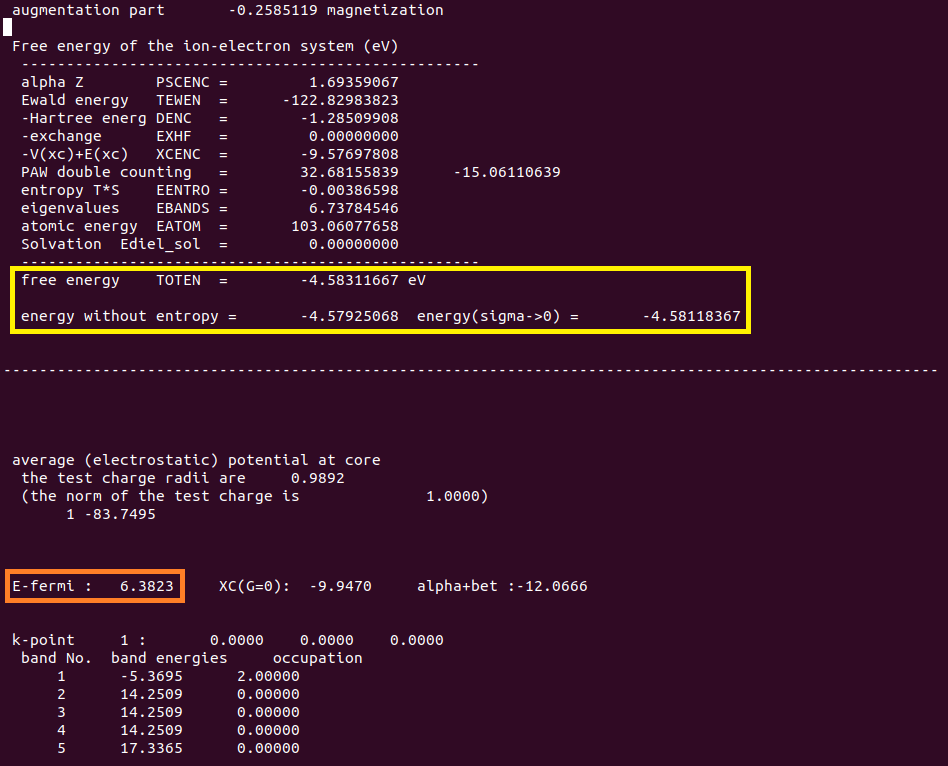
\includegraphics[width=3.5in]{Figures/VASP_example-Si_OUTCAR-2.png}
%\caption{\tiny \textrm{The structure of TiC.}}%(与文献\cite{EPJB33-47_2003}图1对比)
\label{Fig:VASP-Si_OUTCAR-part2}
\end{figure}
}

\frame
{
	\frametitle{\textrm{VASP}计算示范:~\textrm{Si}}
\vspace*{-10pt}
\begin{figure}[h!]
\centering
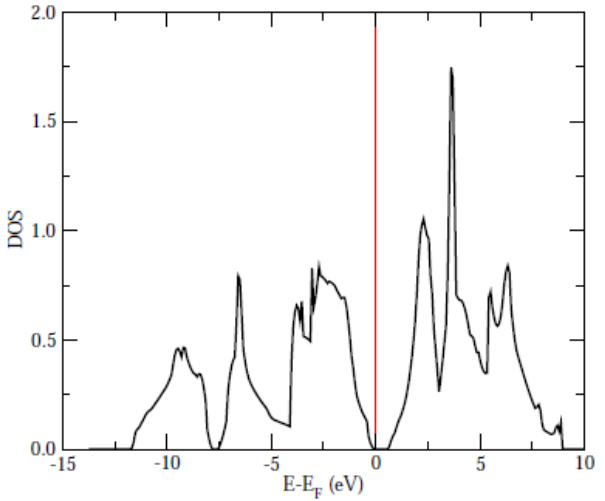
\includegraphics[width=3.5in]{Figures/VASP_cdSi_1.png}
%\caption{\tiny \textrm{The structure of TiC.}}%(与文献\cite{EPJB33-47_2003}图1对比)
\label{Fig:VASP-Si_DOS}
\end{figure}
}

\frame
{
	\frametitle{\textrm{VASP}计算示范:~\textrm{Si}}
%\vspace*{5pt}
\begin{figure}[h!]
\centering
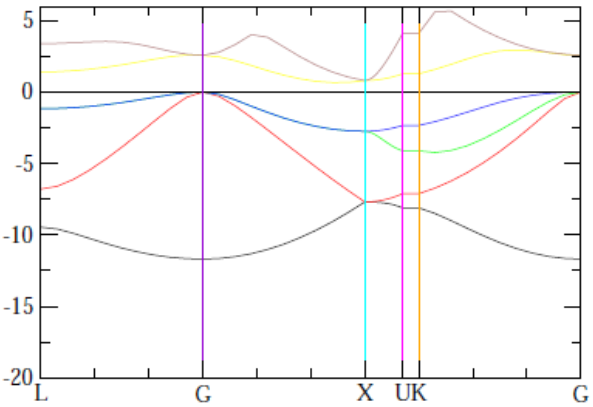
\includegraphics[width=4.0in]{Figures/VASP_cdSi_2.png}
%\caption{\tiny \textrm{The structure of TiC.}}%(与文献\cite{EPJB33-47_2003}图1对比)
\label{Fig:VASP-Si_Band}
\end{figure}
}

\frame
{
	\frametitle{\textrm{VASP}计算示范:~\textrm{Si}}
%\vspace*{5pt}
\begin{figure}[h!]
\centering
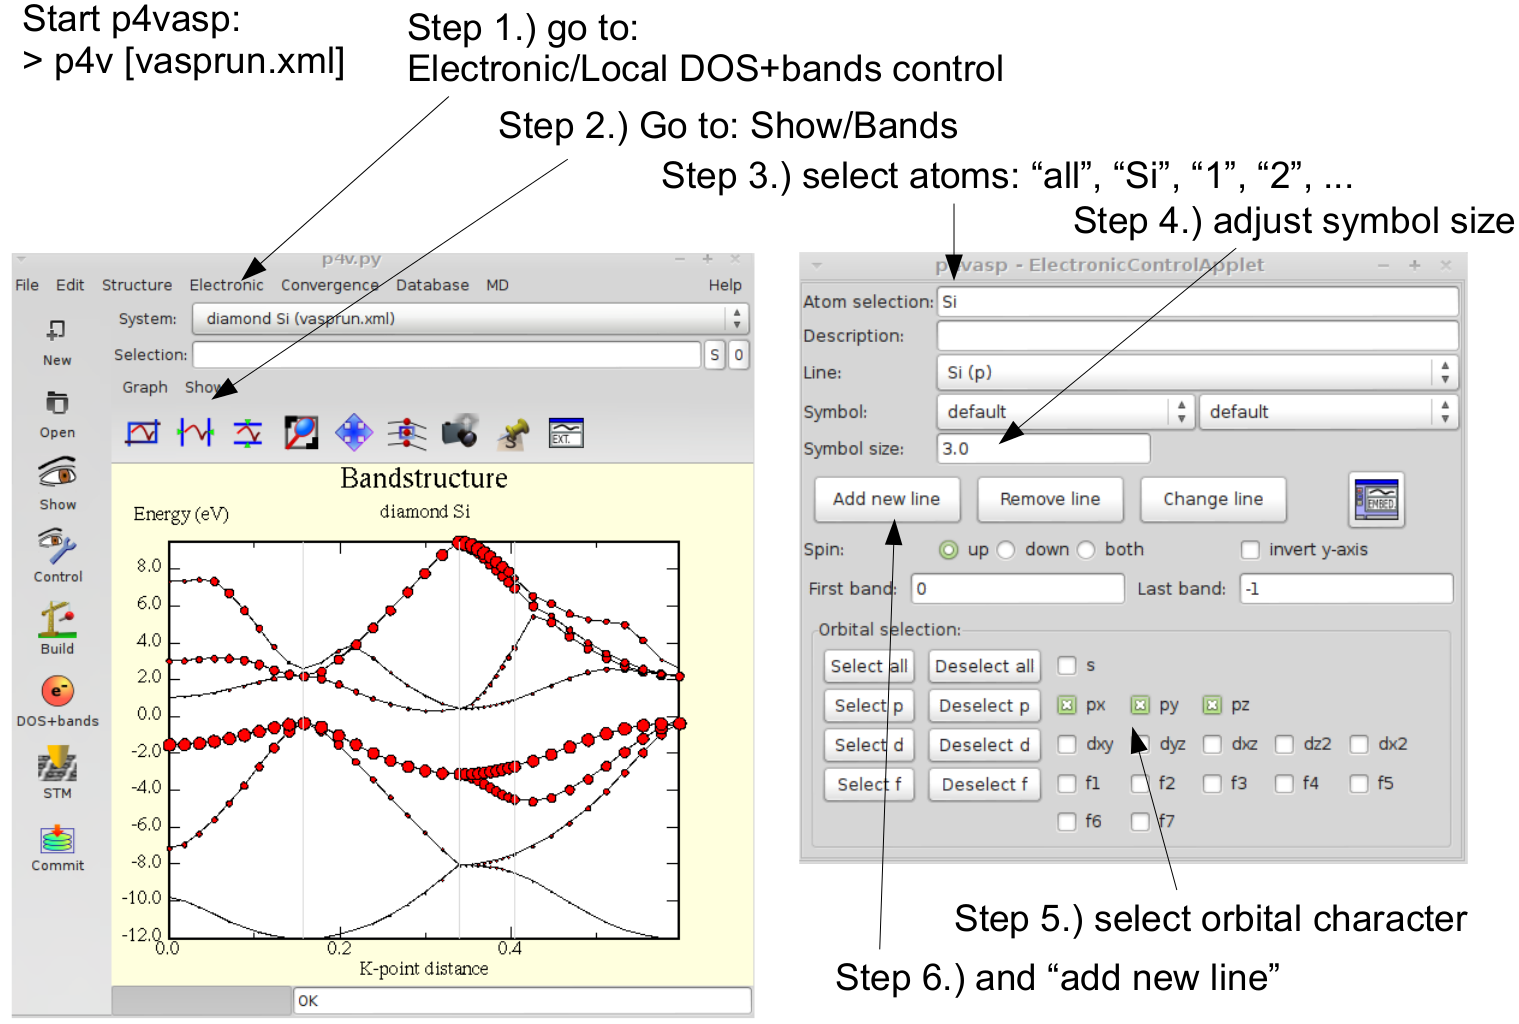
\includegraphics[width=4.0in]{Figures/VASP_cdSi_3.png}
%\caption{\tiny \textrm{The structure of TiC.}}%(与文献\cite{EPJB33-47_2003}图1对比)
\label{Fig:VASP-Si_p4vasp}
\end{figure}
}

\frame
{
	\frametitle{\textrm{WIEN2k}算例:~\textrm{case.structure}}
\vspace*{-17pt}
\begin{minipage}[t]{0.39\textwidth}
\begin{figure}[h!]
\centering
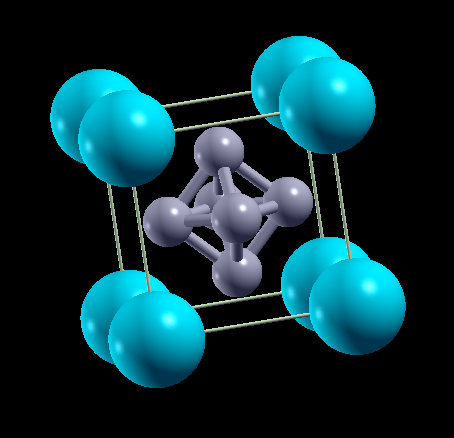
\includegraphics[width=1.5in]{Figures/WIEN2k_CaB6.png}
\caption{\tiny \textrm{The structure of \ch{CaB6}.}}%(与文献\cite{EPJB33-47_2003}图1对比)
\label{Fig:WIEN2k_CaB6}
\end{figure}
\end{minipage}
\hfill
\begin{minipage}[t]{0.59\textwidth}
\begin{figure}[h!]
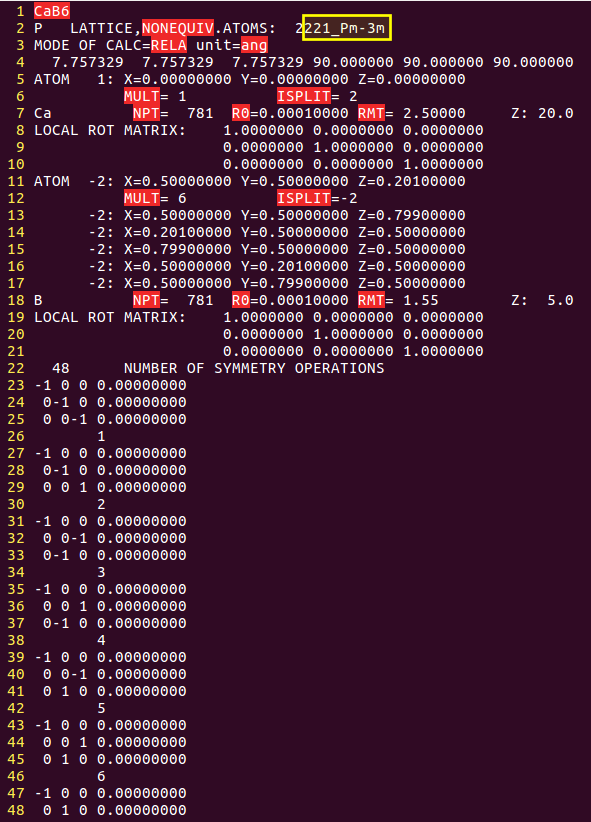
\includegraphics[height=2.95in]{Figures/WIEN2k_CaB6-structure.png}
%\caption{\tiny Breakup of a submesh cell into six tetrahedra.}%(与文献\cite{EPJB33-47_2003}图1对比)
\label{Fig:WIEN2k_CaB6-structure}
\end{figure}
\end{minipage}
}

\frame
{
	\frametitle{\textrm{WIEN2k}计算示范:~\textrm{SCF}}
\vspace*{-13pt}
\begin{figure}[h!]
\centering
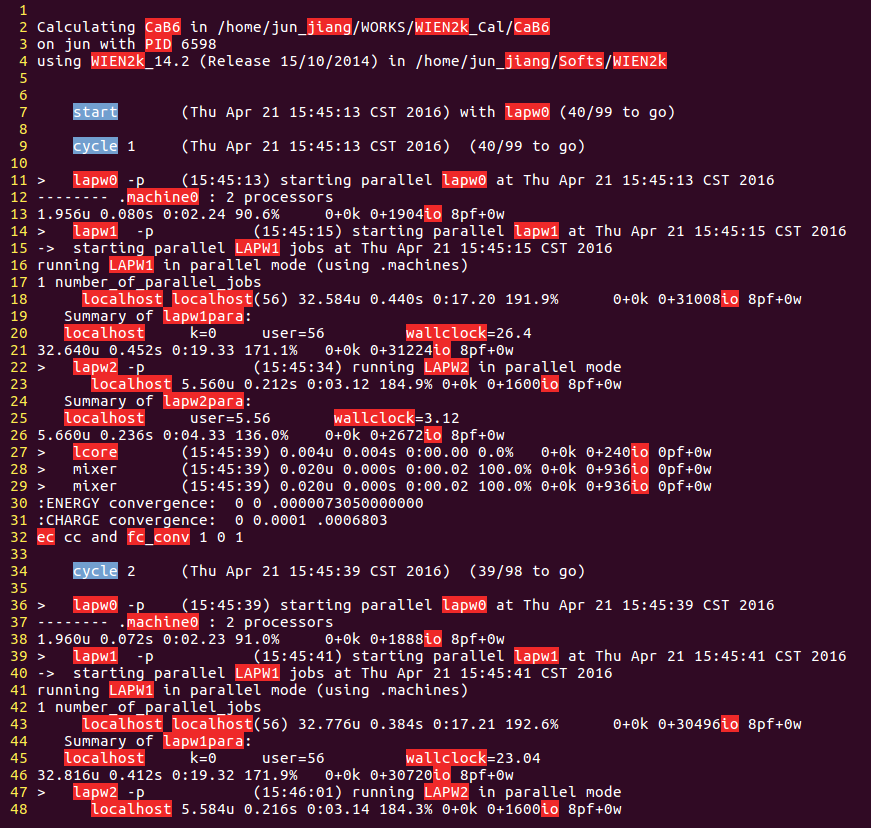
\includegraphics[height=2.98in]{Figures/WIEN2k_CaB6-SCF.png}
%\caption{\tiny \textrm{The structure of TiC.}}%(与文献\cite{EPJB33-47_2003}图1对比)
\label{Fig:WIEN2k_SCF}
\end{figure}
}

\frame
{
	\frametitle{\textrm{WIEN2k}计算示范:~\ch{\textrm{CaB6}}的\textrm{DOS}}
\vspace*{5.0pt}
\begin{figure}[h!]
\centering
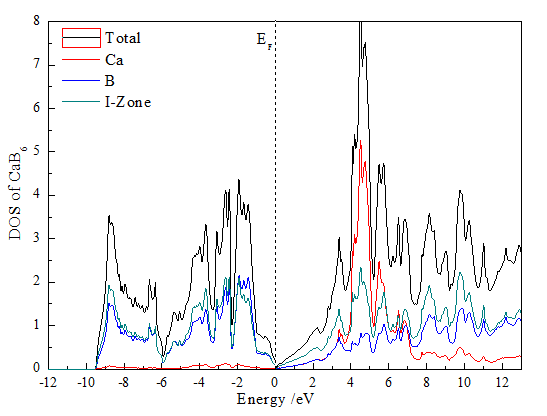
\includegraphics[height=2.30in,width=4.00in]{Figures/WIEN2k_CaB6-DOS.png}
%\caption{\tiny \textrm{The structure of TiC.}}%(与文献\cite{EPJB33-47_2003}图1对比)
\label{Fig:WIEN2k_DOS}
\end{figure}
}

\frame
{
	\frametitle{\textrm{WIEN2k}计算示范:~\ch{\textrm{CaB6}}的能带结构}
\vspace*{-13pt}
\begin{figure}[h!]
\centering
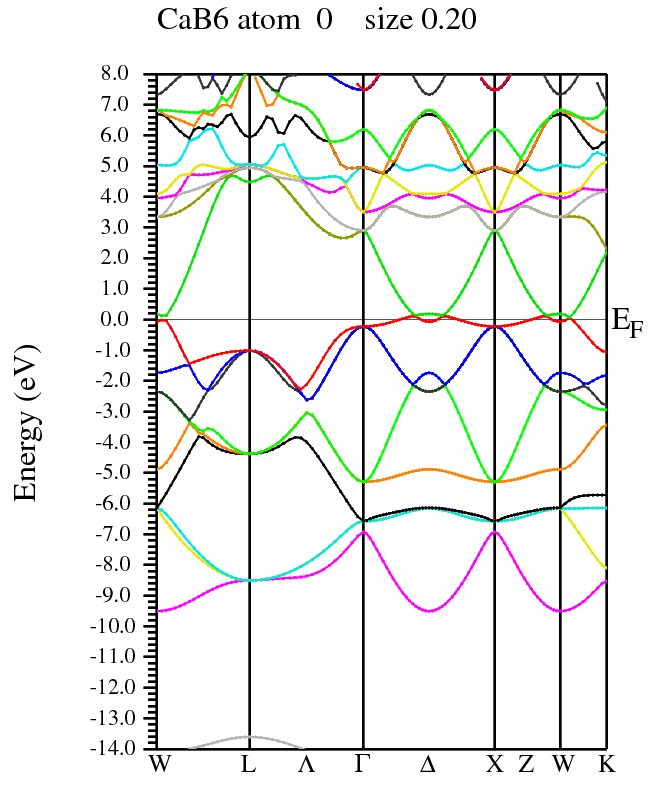
\includegraphics[height=2.98in, viewport=0 10 730 740,clip]{Figures/WIEN2k_CaB6-Band.png}
%\caption{\tiny \textrm{The structure of TiC.}}%(与文献\cite{EPJB33-47_2003}图1对比)
\label{Fig:WIEN2k_Band}
\end{figure}
}

\section{光学性质计算}
\frame
{
	\frametitle{固体光学常数间的基本关系}
	光(电磁波)通过固体材料时,电磁波将与固体中的电子、原子(离子)间相互作用,因此发生光吸收
\begin{figure}[h!]
	\vspace{-3pt}
\centering
\animategraphics[autoplay, loop, height=2.25in, width=3.6in,viewport= 15 30 570 515,clip]{1}{Figures/Light-wave-}{0}{30}
%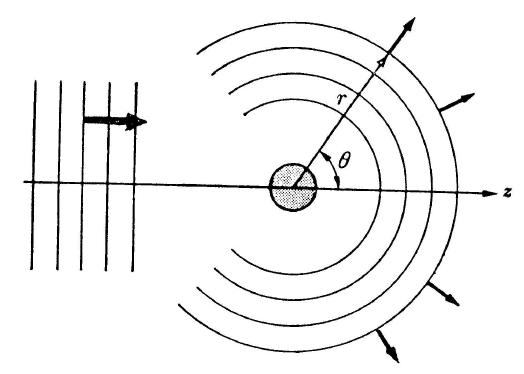
\includegraphics[height=1.29in,width=1.91in,viewport=0 0 400 275,clip]{Figures/Pseudo-scatter.jpg}
\caption{\fontsize{5.5pt}{4.2pt}\selectfont{\textrm{Schematic illustration of electromagnetic wave propagation.}}}%(与文献\cite{EPJB33-47_2003}图1对比)
\label{Light-Wave}
\end{figure}
}

\frame
{
	\frametitle{固体光学常数间的基本关系}
	\begin{itemize}
		\item 电磁波垂直入射时,反射波与入射波分别为
\begin{figure}[h!]
\centering
%\hspace*{-10pt}
\vspace*{-0.4in}
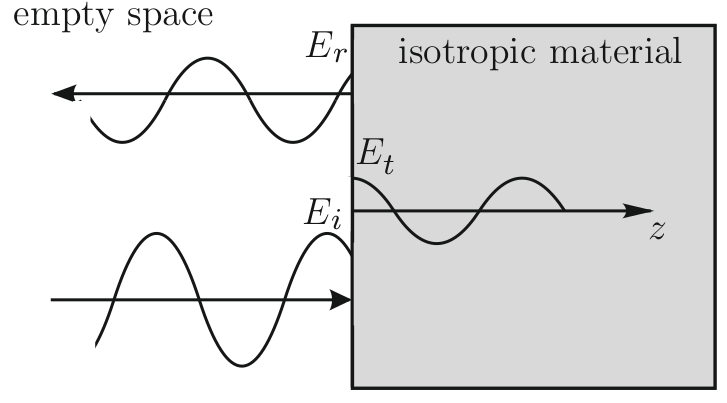
\includegraphics[height=1.2in,width=1.8in,viewport=0 0 750 600,clip]{Figures/Optic-reflect.png}
\caption{\fontsize{5.5pt}{4.2pt}\selectfont{\textrm{Schematic representation of incident, reflected and transmitted electromagnetic\\ wave at the surface.}}}%
\label{Optic-reflect}
\end{figure} 
			\begin{displaymath}
				\begin{aligned}
					&E(z)=E_t\mathrm{e}^{\mathrm{i}(\omega/c)Nz}\quad z>0\\
					&E(z)=E_i\mathrm{e}^{\mathrm{i}(\omega/c)z}+E_r\mathrm{e}^{-\mathrm{i}(\omega/c)z}\quad z<0\\
				\end{aligned}
			\end{displaymath}
			反射率$R$可以表示为
			\begin{displaymath}
				R=\left|\frac{E_r}{E_i}\right|^2=\left|\frac{1-N}{1+N}\right|^2=\frac{(n-1)^2+k^2}{(n+1)^2+k^2}
			\end{displaymath}
	\end{itemize}
}

\subsection{载流子与\rm{Lorentz-Drude}模型}
%\subsection{光子与电子的激发}
\frame
{
	\frametitle{光子与电子的激发}
	电磁波在介质中的传播,伴随了光子与介质中电子的相互作用
\begin{figure}[h!]
\centering
\vspace*{-10pt}
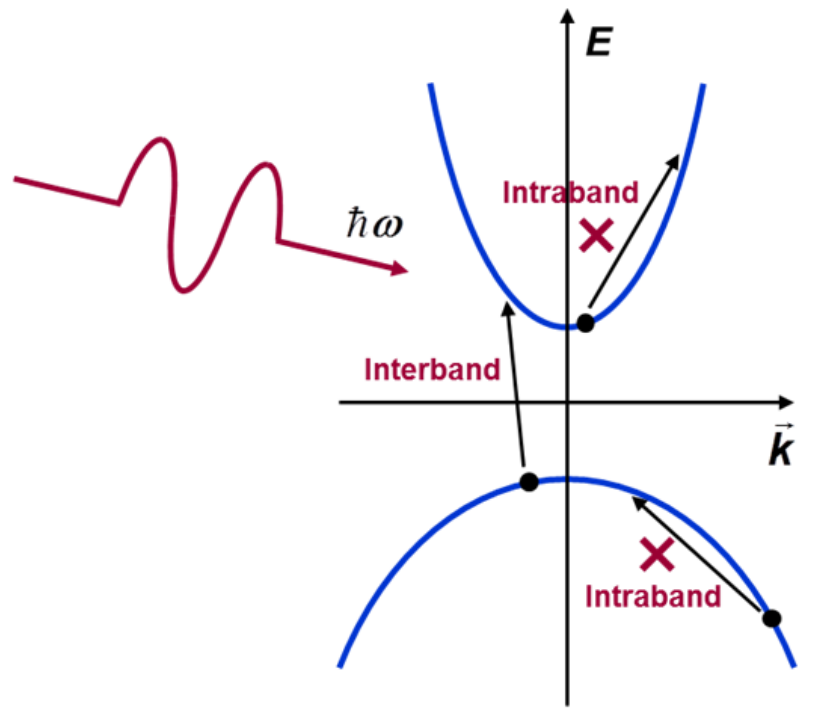
\includegraphics[height=2.3in,width=2.2in,viewport=0 0 800 800,clip]{Figures/Inter-Intra_band-transition.png}
\caption{\fontsize{5.5pt}{4.2pt}\selectfont{\textrm{Schematic representation of interaction of photons and the electrons in the semiconductor.}}}%
\label{Optic-transition}
\end{figure} 
}

\frame
{
	\frametitle{光子与电子的激发}
	粒子间相互作用遵守能量守恒与动量守恒:~\\
	假设介质中的电子初始态为$\vec k_i$,对应的能量为$E_n(\vec k_i)$,电子吸收入射光子跃迁到终态$\vec k_f$,能量变为$E_m(\vec k_f)$,则有
	\begin{itemize}
		\item \textcolor{blue}{能量守恒}
			\begin{displaymath}
				E_m(\vec k_f)=E_n(\vec k_i)+\hbar\omega
			\end{displaymath}
			$\hbar\omega$是入射光子能量
		\item \textcolor{blue}{动量守恒}
			\begin{displaymath}
				\vec k_f=\vec k_i+\vec q
			\end{displaymath}
			$\vec q$是入射光子的动量
	\end{itemize}
	具体计算过程中,考虑光子引起的介质中电子的状态变化,采取了一系列的简化
}

\frame
{
	\frametitle{电场中的自由电子:~\textrm{Lorentz}模型}
	\begin{itemize}
		\item 载流子在外电场$\mathbf{E}(\vec r,t)=\mathbf{E}_0\mathrm{e}^{\mathrm{i}(\vec q\cdot\vec r-\omega t)}$下的运动方程
			\begin{displaymath}
				m\ddot{\vec r}=-\frac m{\tau}\dot{\vec r}+(-e)\mathbf{E}_0\mathrm{e}^{\mathrm{i}(\vec q\cdot\vec r-\omega t)}
			\end{displaymath}
			这里$\vec r(t)$是载流子坐标,$\tau$是\textcolor{red}{唯象弛豫时间}
		\item 长波极限下,忽略电磁波在空间的变化
			\begin{displaymath}
				m\ddot{\vec r}=-\frac m{\tau}\dot{\vec r}-e\mathbf{E}_0\mathrm{e}^{-\mathrm{i}\omega t}
			\end{displaymath}
			取载流子位置函数$\vec r(t)=\vec A_0\mathrm{e}^{-\mathrm{i}\omega t}$,有
			\begin{displaymath}
				\vec A_0=\frac{e\tau}m\frac1{(\omega^2+\mathrm{i}\omega\tau-\omega_0^2)}\mathbf{E}_0
			\end{displaymath}
	\end{itemize}
	经典图像中,介质中载流子的运动可类比于谐振子,$\omega_0$为弹簧的固有频率
}

%\frame
%{
%	\frametitle{\textrm{Lorentz}模型}
%由谐振子偶极与电场的关系(电极化率)可有
%\begin{displaymath}
%\begin{aligned}
%	\mathbf{P}=&N\mathbf{p}\\
%	\mathbf{P}=&\varepsilon_0\chi_{\mathrm{e}}\mathbf{E}\\
%	\varepsilon=&1+\chi_{\mathrm{e}}
%\end{aligned}
%\end{displaymath}
%这里$\chi_{\mathrm{e}}$称为电极化率
%\begin{displaymath}
%\begin{aligned}
%	\vec p=&q\vec r(t)\\
%	=&\dfrac{q^2}m\dfrac1{(\omega^2+\mathrm{i}\omega\tau-\omega_0^2)}\mathbf{E}_0\mathrm{e}^{-\mathrm{i}\omega t}\\
%	=&\dfrac{q^2}m\dfrac1{(\omega^2+\mathrm{i}\omega\tau-\omega_0^2)}\mathbf{E}
%\end{aligned}
%\end{displaymath}
%因此
%\begin{displaymath}
%	\varepsilon=1+\dfrac{Nq^2}{m\varepsilon_0}\dfrac1{(\omega^2+\mathrm{i}\omega\tau-\omega_0^2)}\Longrightarrow \omega_{\mathrm{p}}^2=\dfrac{Nq^2}{m\varepsilon_0}	
%\end{displaymath}
%}
%
\frame
{
	\frametitle{\textrm{Lorentz}模型}
\begin{figure}[h!]
\centering
\vspace*{-5pt}
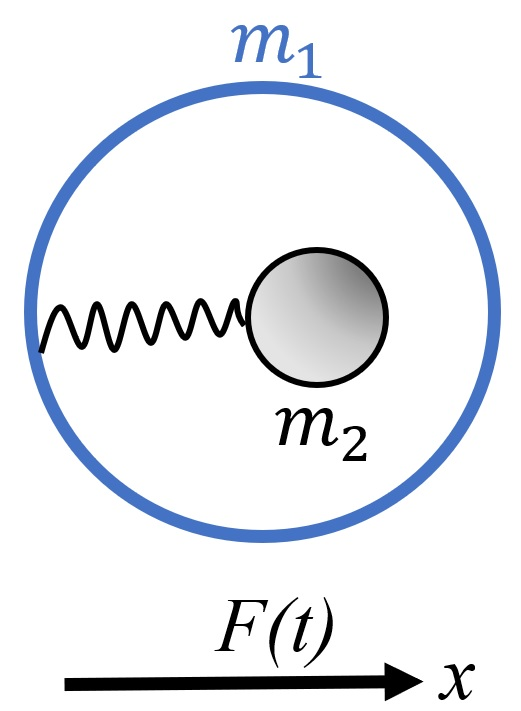
\includegraphics[height=1.05in,width=0.7in,viewport=0 0 380 550,clip]{Figures/A_mechanical_model_giving_rise_to_the_negative_effective_mass_effect.jpg}
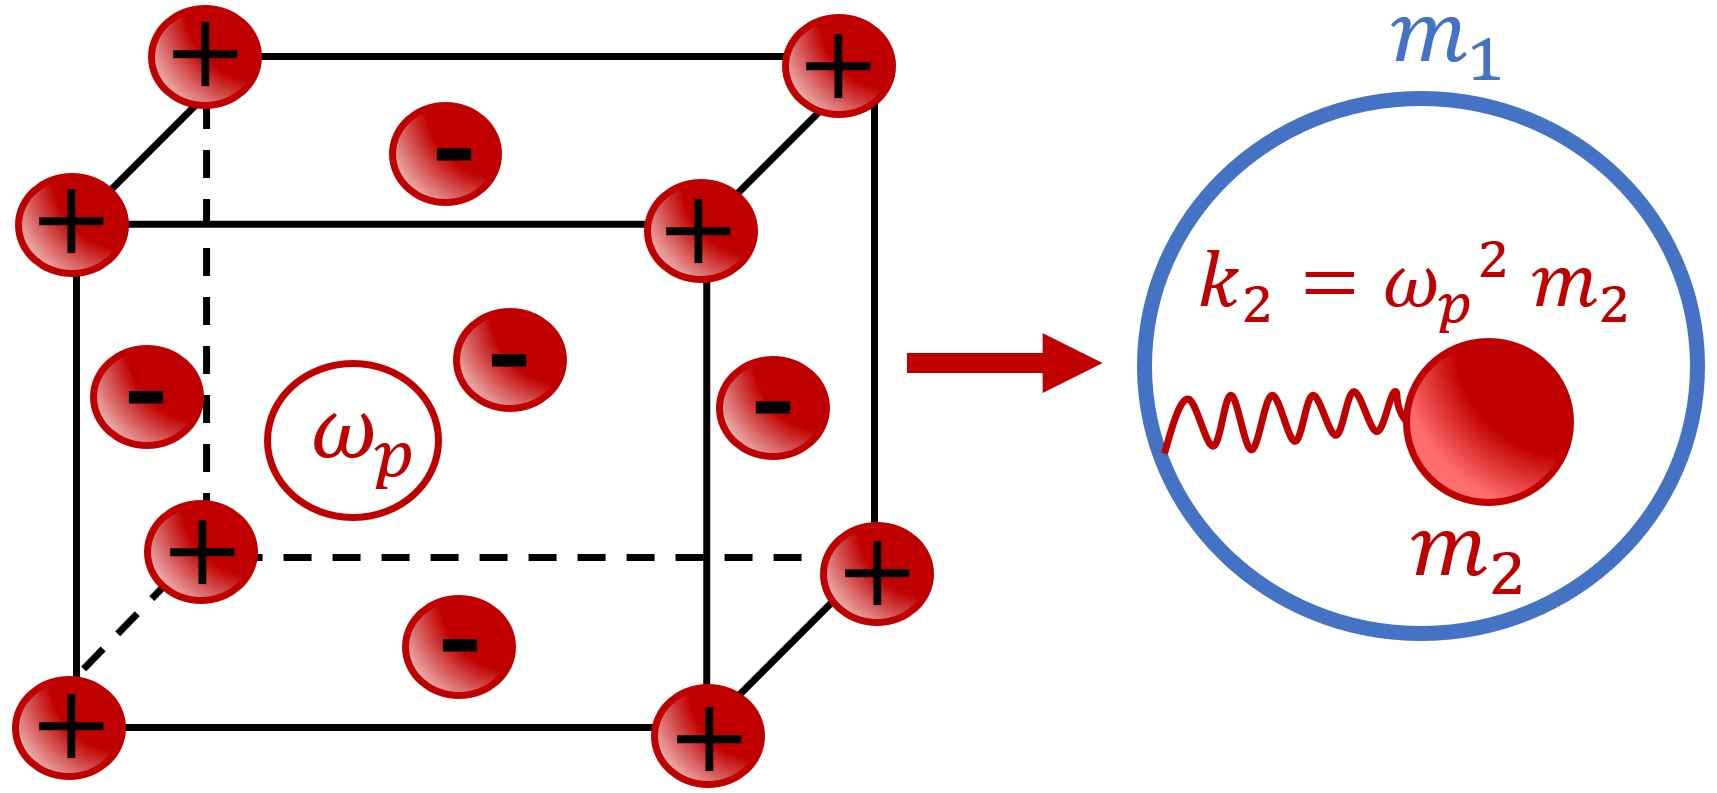
\includegraphics[height=1.55in,width=3.25in,viewport=0 0 1300 600,clip]{Figures/Equivalent_mechanical_scheme_of_electron_gas_in_ionic_lattice.jpg}
\caption{\fontsize{5.5pt}{4.2pt}\selectfont{\textrm{Equivalent mechanical scheme of electron gas in ionic lattice.}}}%
\label{Electron-gas-in-lattice}
\end{figure} 
			$\omega_{\mathrm{p}}$是载流子的等离振荡频率
			\begin{displaymath}
				\omega_{\mathrm{p}}^2=\frac{4\pi ne^2}m
			\end{displaymath}
}

\frame
{
	\frametitle{电场对导带电子的影响}
\begin{figure}[h!]
\centering
\vspace*{-13pt}
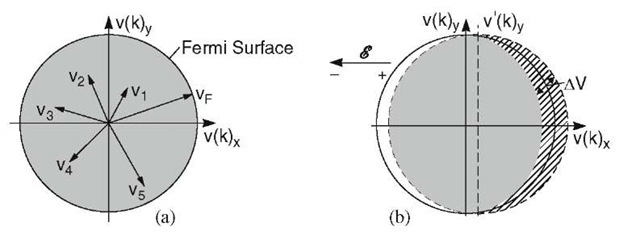
\includegraphics[height=1.4in,width=3.8in,viewport=0 0 480 180,clip]{Figures/Electrmagnetic_Fermi-surface-1.jpg}
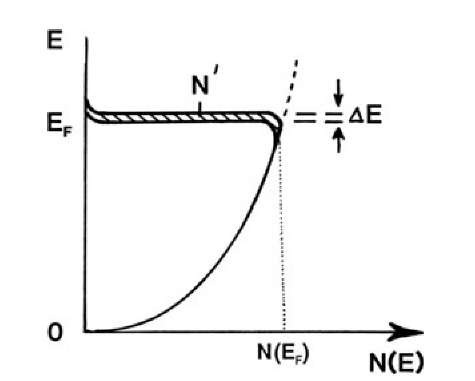
\includegraphics[height=1.35in,width=2.2in,viewport=0 0 200 130,clip]{Figures/Electrmagnetic_Fermi-surface-2.jpg}
\caption{\fontsize{5.5pt}{4.2pt}\selectfont{\textrm{Schematic representation of the Fermi-surface affected by the electrmagnetic field.}}}%
\label{CB-Electron-in-E}
\end{figure} 
}

\frame
{
	\frametitle{\textrm{Lorentz-Drude}模型}
\begin{itemize}
	\item \textrm{Lorentz-Model}:\\
		始于电子与晶格离子间作用,侧重描述电子在固体中的运动,介电函数为
		\begin{displaymath}
			\varepsilon(\omega)=1-\dfrac{\omega_{\mathrm{p}^2}}{\omega^2+\mathrm{i}\omega\tau-\omega_0^2}
		\end{displaymath}
		\textcolor{blue}{\textrm{Lorentz}模型中,取$\omega_0=0$,即为\textrm{Drude}模型}
	\item \textrm{Drude-Model}:\\
		侧重描述自由电子气对外部交变电场的响应,则介电函数可以表示为:
			\begin{displaymath}
				\varepsilon(\omega)=1-\frac{\omega_\mathrm{p}^2}{\omega(\omega+\mathrm{i}/\tau)}=\underline{\textcolor{blue}{\left[ 1-\frac{\omega_{\mathrm{p}}^2\tau^2}{1+\omega^2\tau^2} \right]}}+\mathrm{i}\underline{\textcolor{blue}{\left[ \frac{\omega_{\mathrm{p}}^2\tau}{\omega(1+\omega^2\tau^2)} \right]}}
			\end{displaymath}
%\begin{displaymath}
\end{itemize}
}

\frame
{
	\frametitle{\textrm{Lorentz-Drude}模型}
\begin{figure}[h!]
\centering
\vspace*{-13pt}
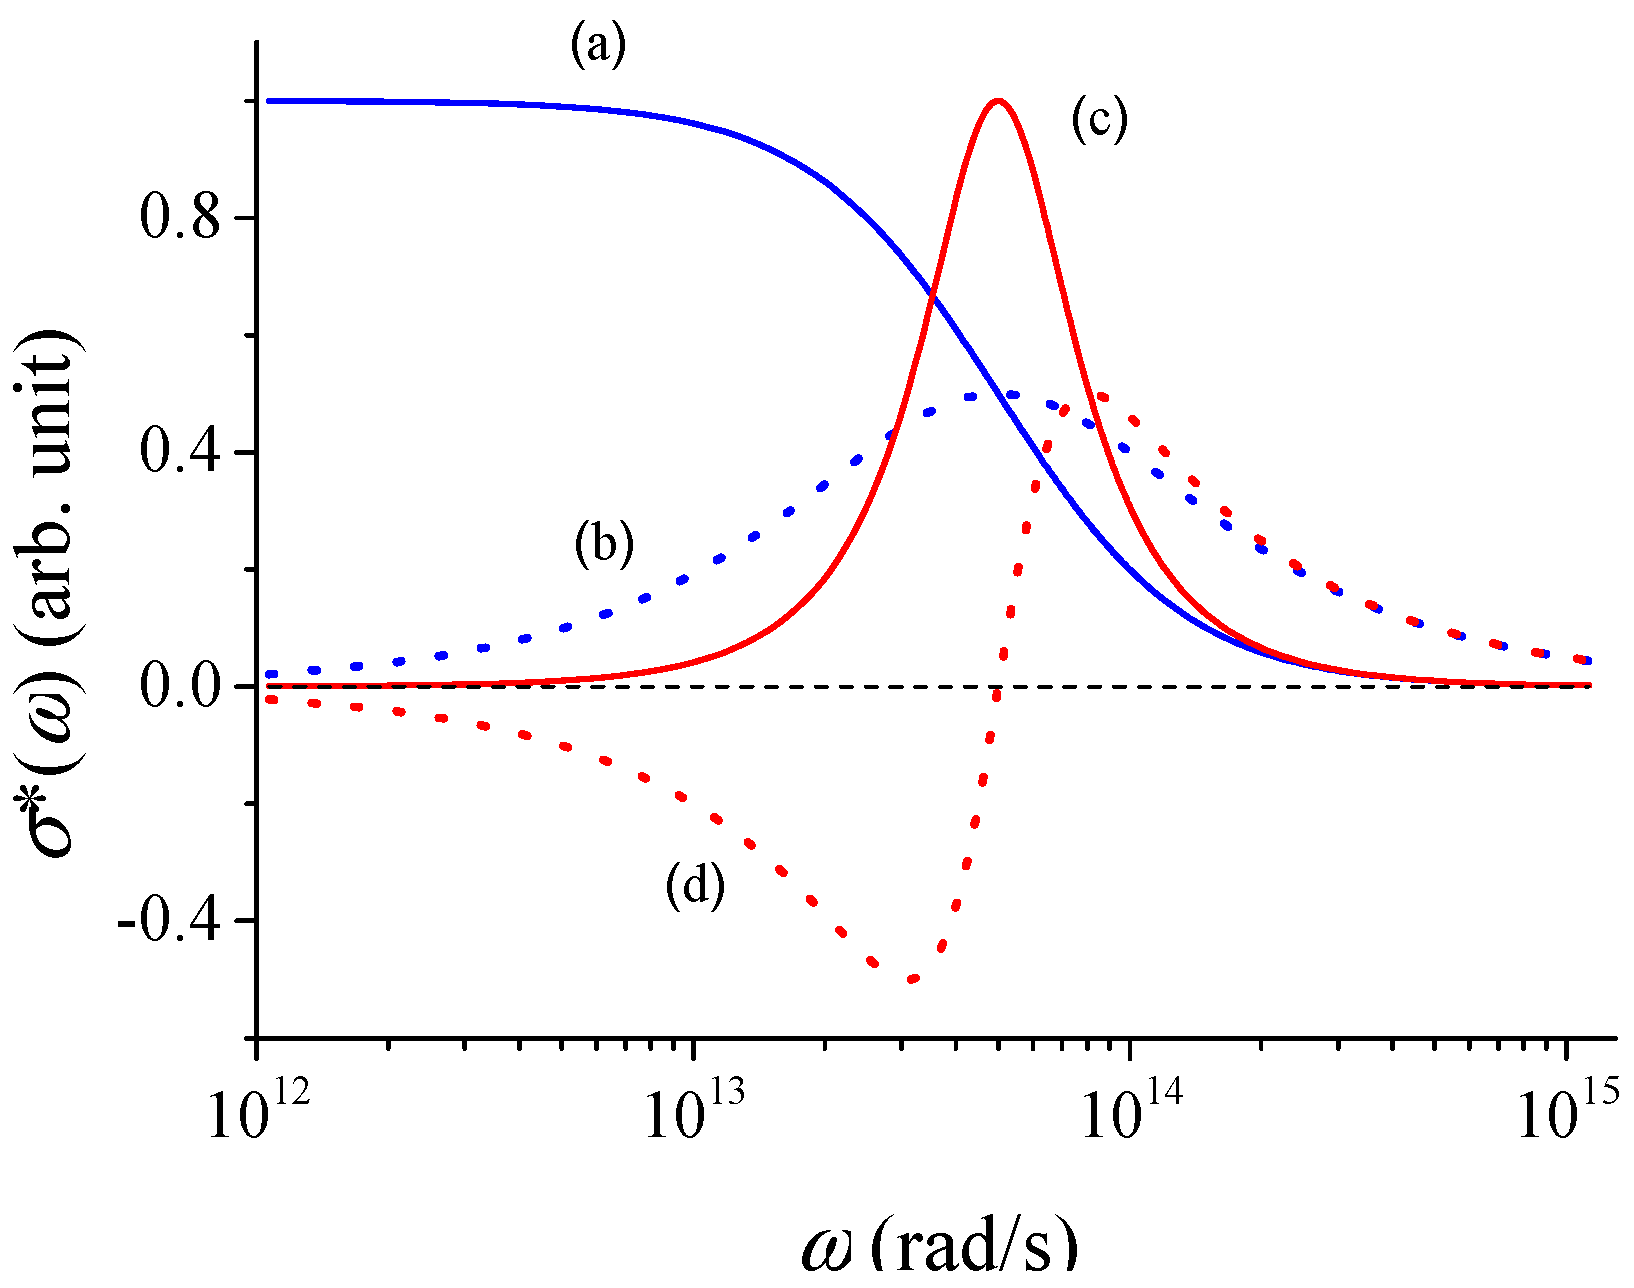
\includegraphics[height=2.5in,width=3.6in,viewport=0 0 200 155,clip]{Figures/Optical-conductivity-in-the-Drude-relaxation-and-in-the-Lorentz-resonance.png}
\caption{\fontsize{5.5pt}{4.2pt}\selectfont{\textrm{Optical conductivity in the Drude relaxation and in the Lorentz resonance.}}}%
\label{Drude-vs-Lorentz}
\end{figure} 
}

\frame
{
	\frametitle{\textrm{Drude}模型}
	\textcolor{blue}{在远红外区,经典自由电子气模型可以很好地描述金属的光学行为}
	如果载流子密度为$n$,则电流密度
	\begin{displaymath}
		\mathbf{J}=n(-e)\dot{\vec r}=n(-e)(-\mathrm{i}\omega)\vec A_0\mathrm{e}^{-\mathrm{i}\omega t}=\frac{ne^2\tau}m\frac1{1-\mathrm{i}\omega\tau}\mathbf{E}_0\mathrm{e}^{-\mathrm{i}\omega t}
	\end{displaymath}
	由此可得频率有关的电导率表示为
	\begin{displaymath}
		\sigma(\omega)=\frac{ne^2\tau}m\frac1{1-\mathrm{i}\omega\tau}=\sigma_0\frac1{1-\mathrm{i}\omega\tau}
	\end{displaymath}
	其中$\sigma_0=ne^2\tau/m$是静态电导率
%	\begin{itemize}
%		\item 
	介电函数可表示为
	\begin{displaymath}
	\epsilon_1(\omega)=1-\frac{\omega_{\mathrm{p}}^2\tau^2}{1+\omega^2\tau^2}\quad \epsilon_2(\omega)=\frac{\omega_{\mathrm{p}}^2\tau}{\omega(1+\omega^2\tau^2)}\quad
\end{displaymath}
%	\end{itemize}
}

\frame
{
\frametitle{带间跃迁的计算}
\begin{itemize}
\setlength{\itemsep}{10pt}
	\item 用半经典方法处理周期性体系的光学性质,用量子力学处理介质,对电磁波仍然采用经典电动力学描写
	\item 以半导体中的带间垂直跃迁(价带$|v,\vec k\rangle$,导带$|c,\vec k\rangle$)为例讨论固体的能带间跃迁
\begin{figure}[h!]
\centering
%\hspace*{-10pt}
\vspace*{-0.2in}
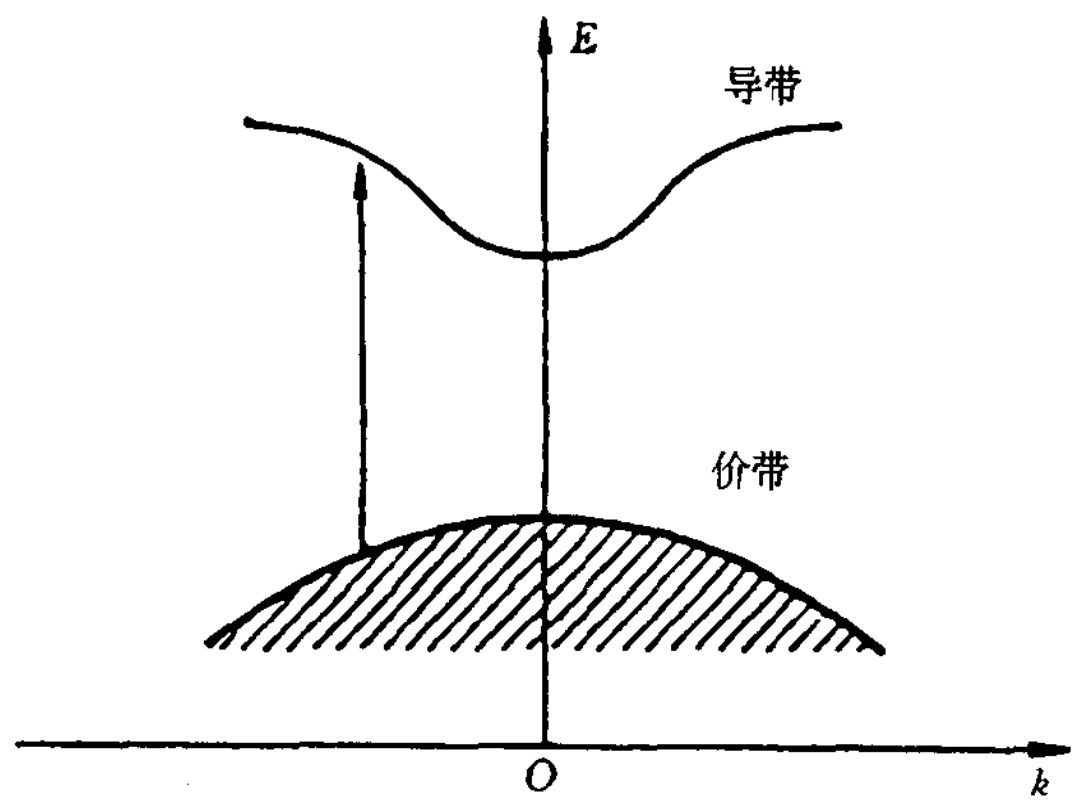
\includegraphics[height=1.8in,width=2.0in,viewport=0 0 1000 900,clip]{Figures/optic_dir.png}
\caption{\fontsize{8.0pt}{5.2pt}\selectfont\textrm{Schematic representation of directly inter-band transition.}}%
\label{Optic-dir}
\end{figure} 
\end{itemize}
}

\frame
{
	\frametitle{带间跃迁的计算}
长波极限下($\vec q\rightarrow0$), 根据光学性质的基本关系,可有介电函数的介电函数虚部表达式
\begin{displaymath}
	\begin{aligned}
		\varepsilon_2(\omega)=&\lim_{\vec q\rightarrow0}\frac{8\pi^2e^2}{m_e^2\omega^2}\int\frac{\mathrm{d}\vec k}{(2\pi)^3}|\langle c,\vec k|\mathbf{e}\cdot\vec p|v,\vec k\rangle|^2\\
		\times&\delta(E_c(\vec k)-E_v(\vec k)-\hbar\omega)[f(E_c(\vec k))-f(E_v(\vec k))]
	\end{aligned}
  \label{eq:optic-varepsilon_2}
\end{displaymath}
$\varepsilon_2(\omega)$是晶体的光学吸收和能带结构之间的基本关系

对应的$\varepsilon_1$可以根据\textrm{Kramers-Kr\"onig}关系%\eqref{eq:optic-16}
得到
\begin{displaymath}
	\varepsilon_1(\omega)=1+\frac1{\pi}\mathscr{P}\int_{-\infty}^{+\infty}\frac{\varepsilon_2(\omega^{\prime})}{\omega^{\prime}-\omega}\textrm{d}\omega^{\prime}=1+\frac2{\pi}\mathscr{P}\int_0^{+\infty}\frac{\omega^{\prime}\varepsilon_2(\omega^{\prime})}{\omega^{\prime2}-\omega^2}\textrm{d}\omega^{\prime}
  \label{eq:optic-varepsilon_1}
\end{displaymath}
因此介电函数表示为
\begin{displaymath}
	\hspace*{-10pt}
	\varepsilon(\omega)=1+\frac{8\pi e^2}{m_e^2}\int\frac{\mathrm{d}\vec k}{(2\pi)^3}\frac{|\langle c,\vec k|\mathbf{e}\cdot\vec p|v,\vec k\rangle|^2}{(E_c(\vec k)-E_v(\vec k))/\hbar^2}\frac{(-\mathrm{i})[f(E_c(\vec k))-f(E_v(\vec k))]}{E_c(\vec k)-E_v(\vec k)-\hbar\omega-\mathrm{i}\eta}
  \label{eq:optic-varepsilon}
\end{displaymath}
}

\frame
{
	\frametitle{带间跃迁和带内跃迁的计算}
电导率函数可表示为
\begin{displaymath}
	\sigma(\omega)=\frac{2e^2}{m_e^2}\int\frac{\mathrm{d}\vec k}{(2\pi)^3}\frac{|\langle c,\vec k|\mathbf{e}\cdot\vec p|v,\vec k\rangle|^2}{(E_c(\vec k)-E_v(\vec k))/\hbar}\frac{(-\mathrm{i})[f(E_c(\vec k))-f(E_v(\vec k))]}{E_c(\vec k)-E_v(\vec k)-\hbar\omega-\mathrm{i}\eta}
  \label{eq:optic-sigma}
\end{displaymath}

\textcolor{violet}{推广到长波极限下的带内跃迁}
\begin{displaymath}
	f(E_c(\vec k))-f(E_v(\vec k))\approx\frac{\partial f}{\partial E}(f(E_c(\vec k))-f(E_v(\vec k)))
\end{displaymath}
\begin{displaymath}
	\sigma(\omega)=\frac{e^2\hbar}{4\pi^3}\int\mathrm{d}\vec k\langle c,\vec k|\mathbf{e}\cdot\vec p|v,\vec k\rangle|^2\frac{-\mathrm{i}}{E_c(\vec k)-E_v(\vec k)-\hbar\omega-\mathrm{i}\eta}\left( -\frac{\partial f}{\partial E} \right)
\end{displaymath}
引入等式$\eta=\hbar/\tau$,并作展开
\begin{displaymath}
	E_{\vec k+\vec q}-E_{\vec k}\approx\vec q\cdot(\partial E/\partial\vec k)=\frac{\hbar}{m_e}\langle c,\vec k|\mathbf{q}\cdot\vec p|v,\vec k\rangle
\end{displaymath}
由此可得
\vspace{-5pt}
\begin{displaymath}
	\sigma(\vec q,\omega)=\frac{e^2}{4\pi^3}\int\mathrm{d}\vec k\frac{\tau|\langle c,\vec k|\mathbf{e}\cdot\vec p|v,\vec k\rangle|^2}{1-\mathrm{i}\tau(\omega-\langle c,\vec k|\mathbf{q}\cdot\vec p|v,\vec k\rangle)}\left( -\frac{\partial f}{\partial E} \right)
\end{displaymath}
}

\frame
{
	\frametitle{\textrm{WIEN2k}计算示范:~光学性质计算}
\vspace*{-5pt}
\begin{figure}[h!]
\centering
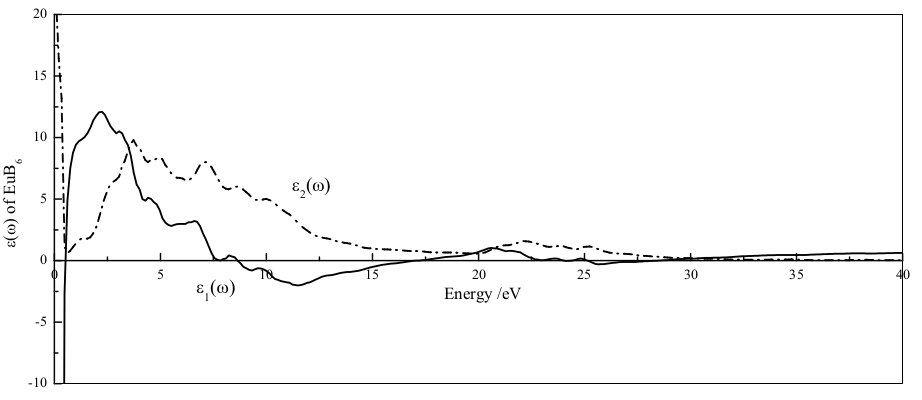
\includegraphics[width=4.15in]{Figures/WIEN2k_EuB6-epsil.png}
\caption{\tiny \textrm{The dielectric of \ch{EuB6}.}}%(与文献\cite{EPJB33-47_2003}图1对比)
\label{Fig:WIEN2k_EuB6-dielectric}
\end{figure}
}

\frame
{
	\frametitle{\textrm{WIEN2k}计算示范:~光学性质计算}
\vspace*{-5pt}
\begin{figure}[h!]
\centering
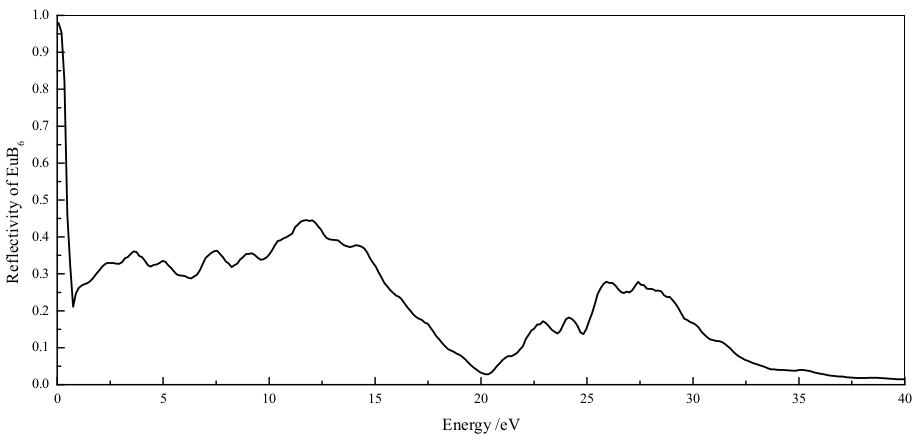
\includegraphics[width=4.15in]{Figures/WIEN2k_EuB6-Reflect.png}
\caption{\tiny \textrm{The Reflectivity of \ch{EuB6}.}}%(与文献\cite{EPJB33-47_2003}图1对比)
\label{Fig:WIEN2k_EuB6-Reflectivity}
\end{figure}
}

\frame
{
	\frametitle{\textrm{WIEN2k}计算示范:~光学性质计算}
\vspace*{-5pt}
\begin{figure}[h!]
\centering
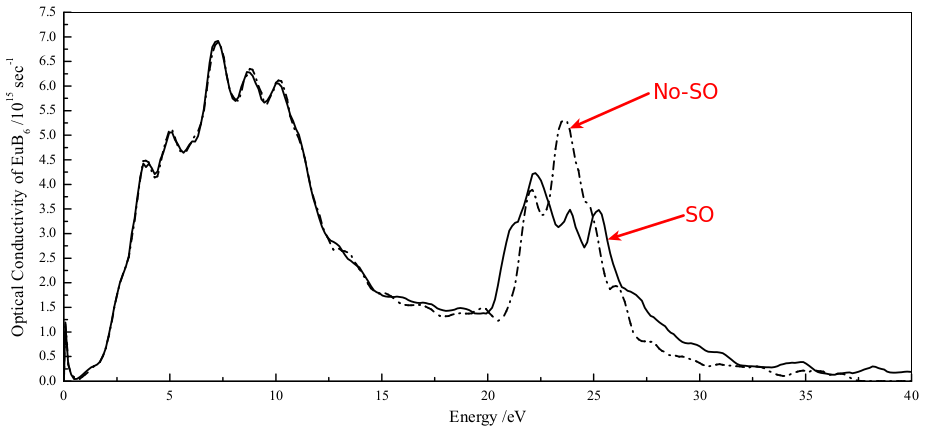
\includegraphics[width=4.15in]{Figures/WIEN2k_EuB6-Conduct.png}
\caption{\tiny \textrm{The R-conductivity of \ch{EuB6}.}}%(与文献\cite{EPJB33-47_2003}图1对比)
\label{Fig:WIEN2k_EuB6-conductivity}
\end{figure}
}

\frame
{
	\frametitle{\textrm{WIEN2k}计算示范:~光学性质计算}
\vspace*{-5pt}
\begin{figure}[h!]
\centering
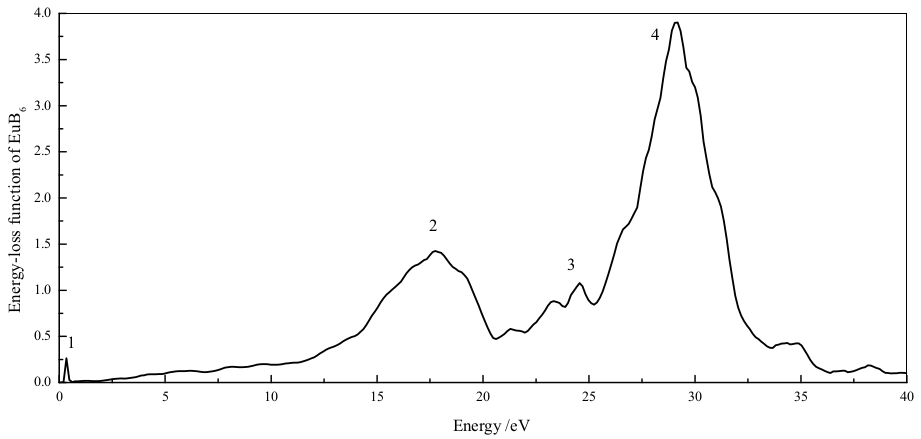
\includegraphics[width=4.15in]{Figures/WIEN2k_EuB6-eloss.png}
\caption{\tiny \textrm{The E-loss function of \ch{EuB6}.}}%(与文献\cite{EPJB33-47_2003}图1对比)
\label{Fig:WIEN2k_EuB6-eloss}
\end{figure}
}

%\subsection{复杂的光子与电子相互作用}
\frame
{
	\frametitle{电子对光子的吸收与受激辐射}
电子、空穴与相互作用	
\begin{figure}[h!]
\centering
%\hspace*{-10pt}
\vspace*{-0.2in}
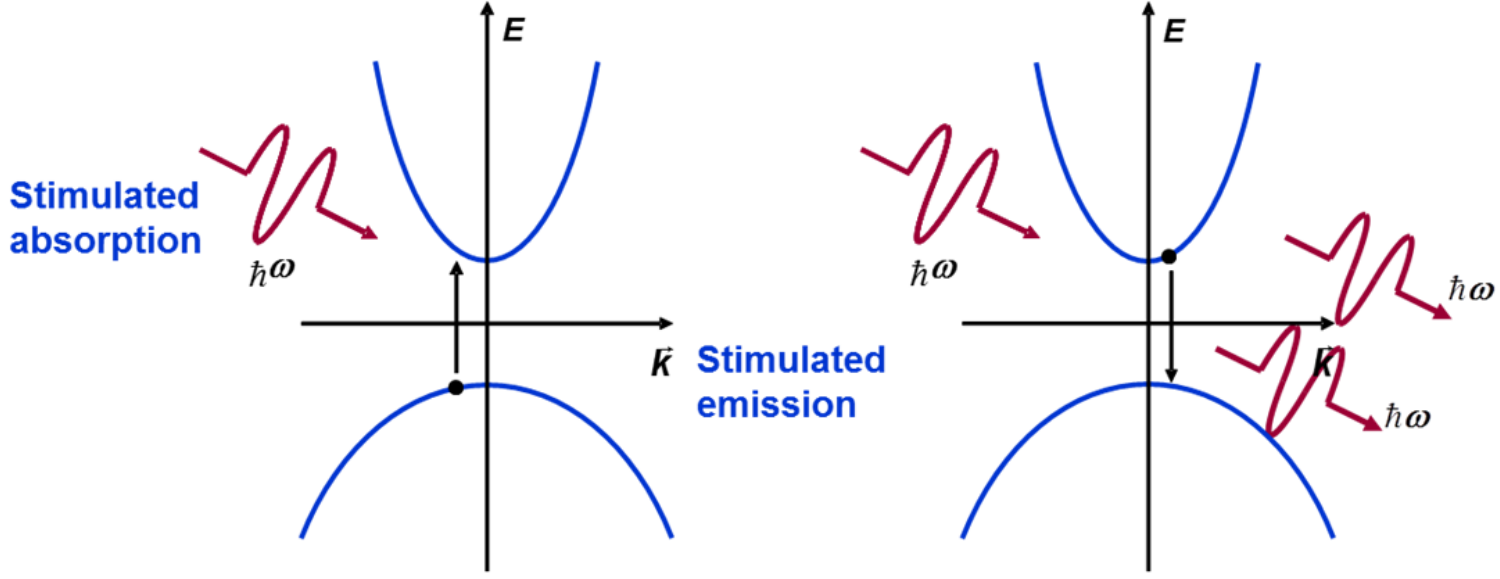
\includegraphics[height=1.9in,width=4.1in,viewport=0 0 1500 600,clip]{Figures/Inter_band-transition_abs-emi.png}
\caption{\fontsize{5.2pt}{4.0pt}\selectfont\textrm{Schematic representation of the stimulated absorption and emission of electrons.}}%
\label{Stimulated-absorption-emission}
\end{figure} 
电子-空穴对构成准粒子\textrm{(quasi-particle)}
}

\frame
{
	\frametitle{电子的自发辐射}
	电子-空穴的复合与准粒子的寿命
\begin{figure}[h!]
\centering
%\hspace*{-10pt}
\vspace*{-0.05in}
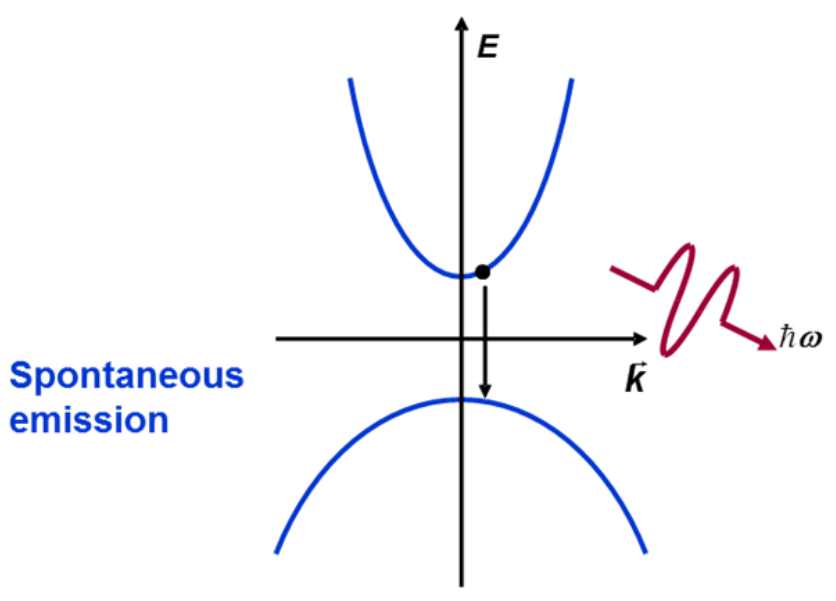
\includegraphics[height=2.0in,width=2.7in,viewport=0 0 830 620,clip]{Figures/Inter_band-transition_emission.png}
\caption{\fontsize{5.2pt}{4.0pt}\selectfont\textrm{Schematic representation of the spontaneous emission of electrons.}}%
\label{spontaneous-emission}
\end{figure} 
}

\frame
{
	\frametitle{吸收谱与发射谱}
\begin{figure}[h!]
\centering
%\hspace*{-10pt}
\vspace*{-0.19in}
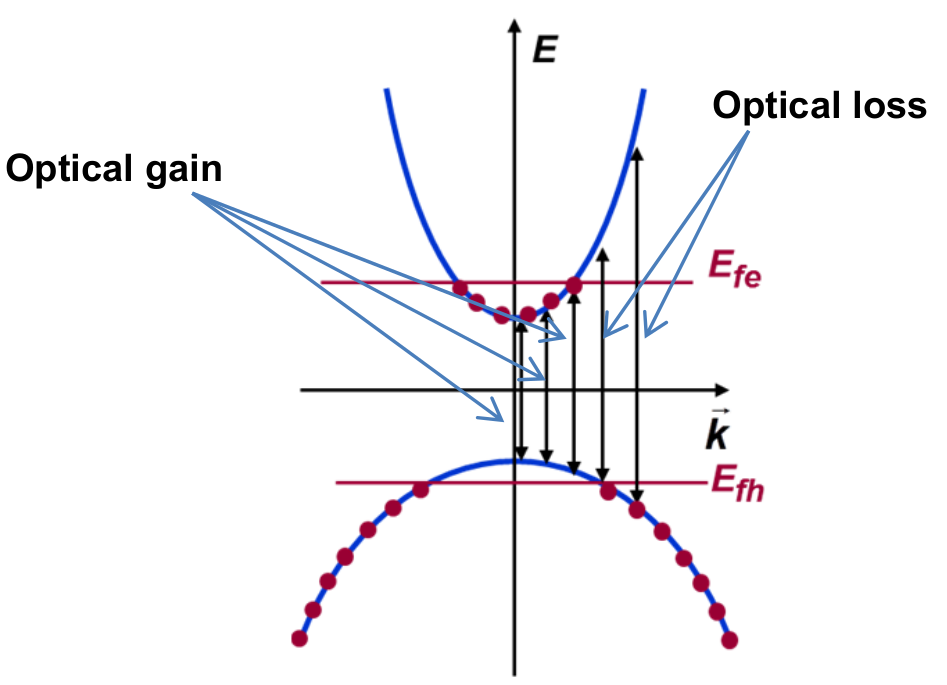
\includegraphics[height=2.5in,width=3.80in,viewport=0 0 950 700,clip]{Figures/Optical_gain-loss.png}
%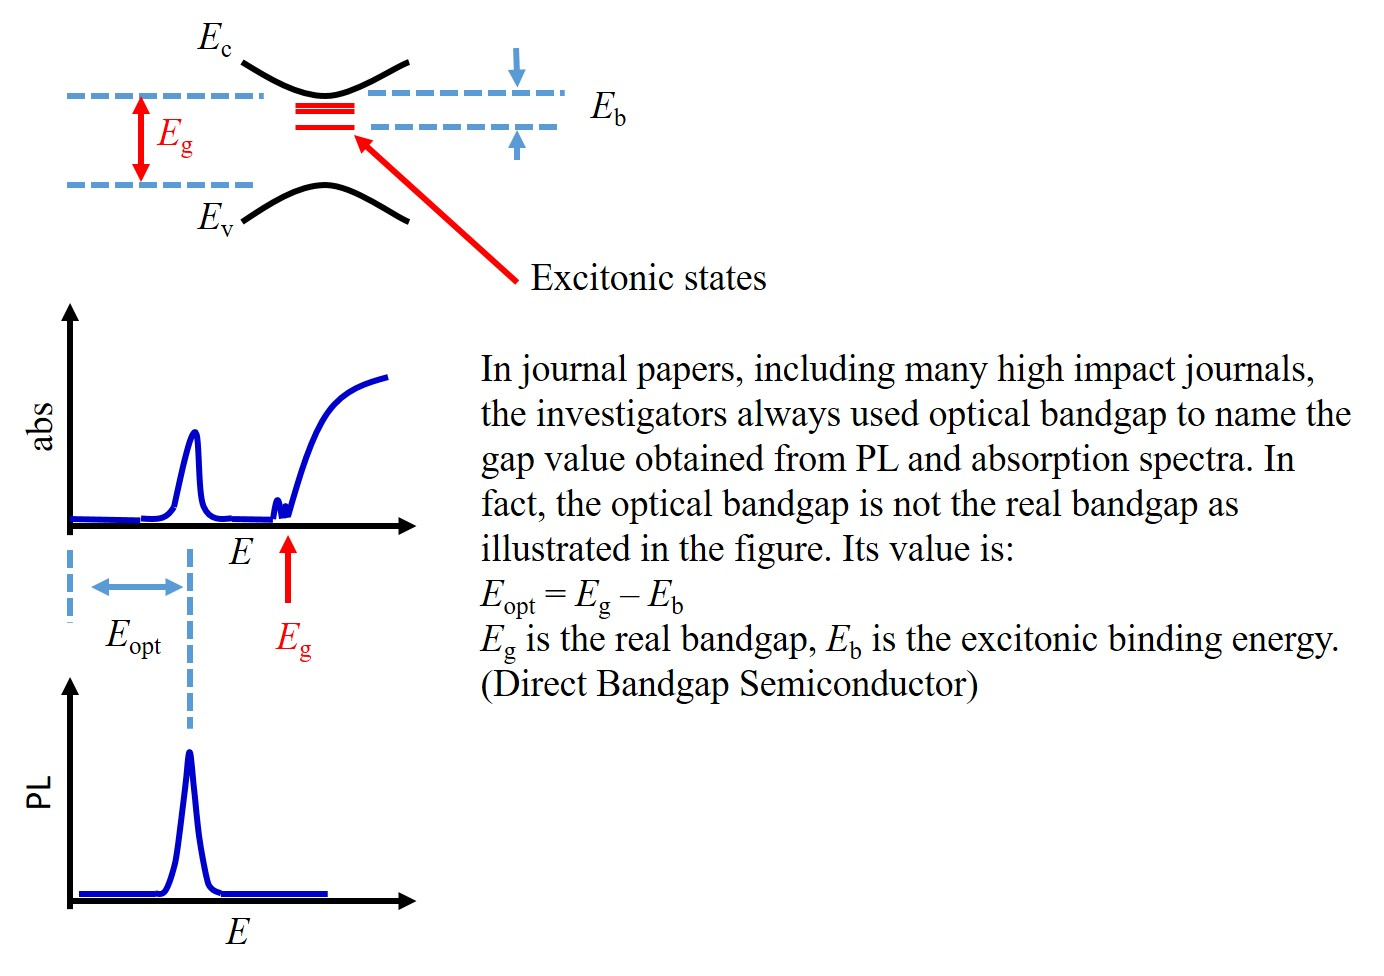
\includegraphics[height=1.1in,width=2.00in,viewport=0 0 670 460,clip]{Figures/Optical_Bandgap.jpg}
\caption{\fontsize{5.2pt}{4.0pt}\selectfont\textrm{Schematic representation of the gain-loss spectra.}}%
\label{gain-loss_Bandgap}
\end{figure} 
}

\frame
{
	\frametitle{光电子能谱与电子带隙}
\begin{figure}[h!]
\centering
%\hspace*{-10pt}
\vspace*{-3pt}
%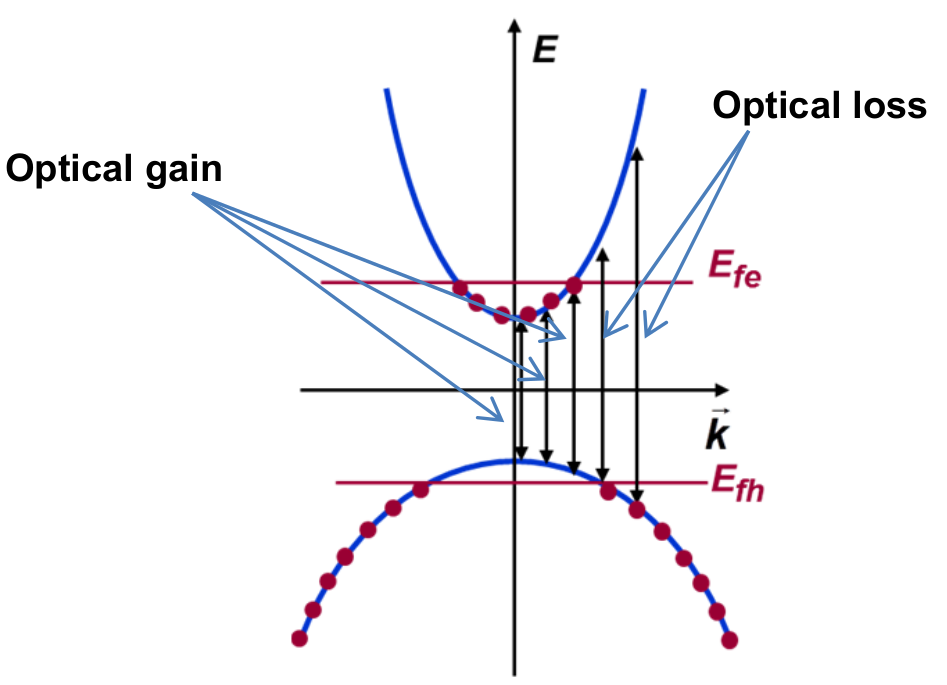
\includegraphics[height=1.7in,width=2.30in,viewport=0 0 950 700,clip]{Figures/Optical_gain-loss.png}
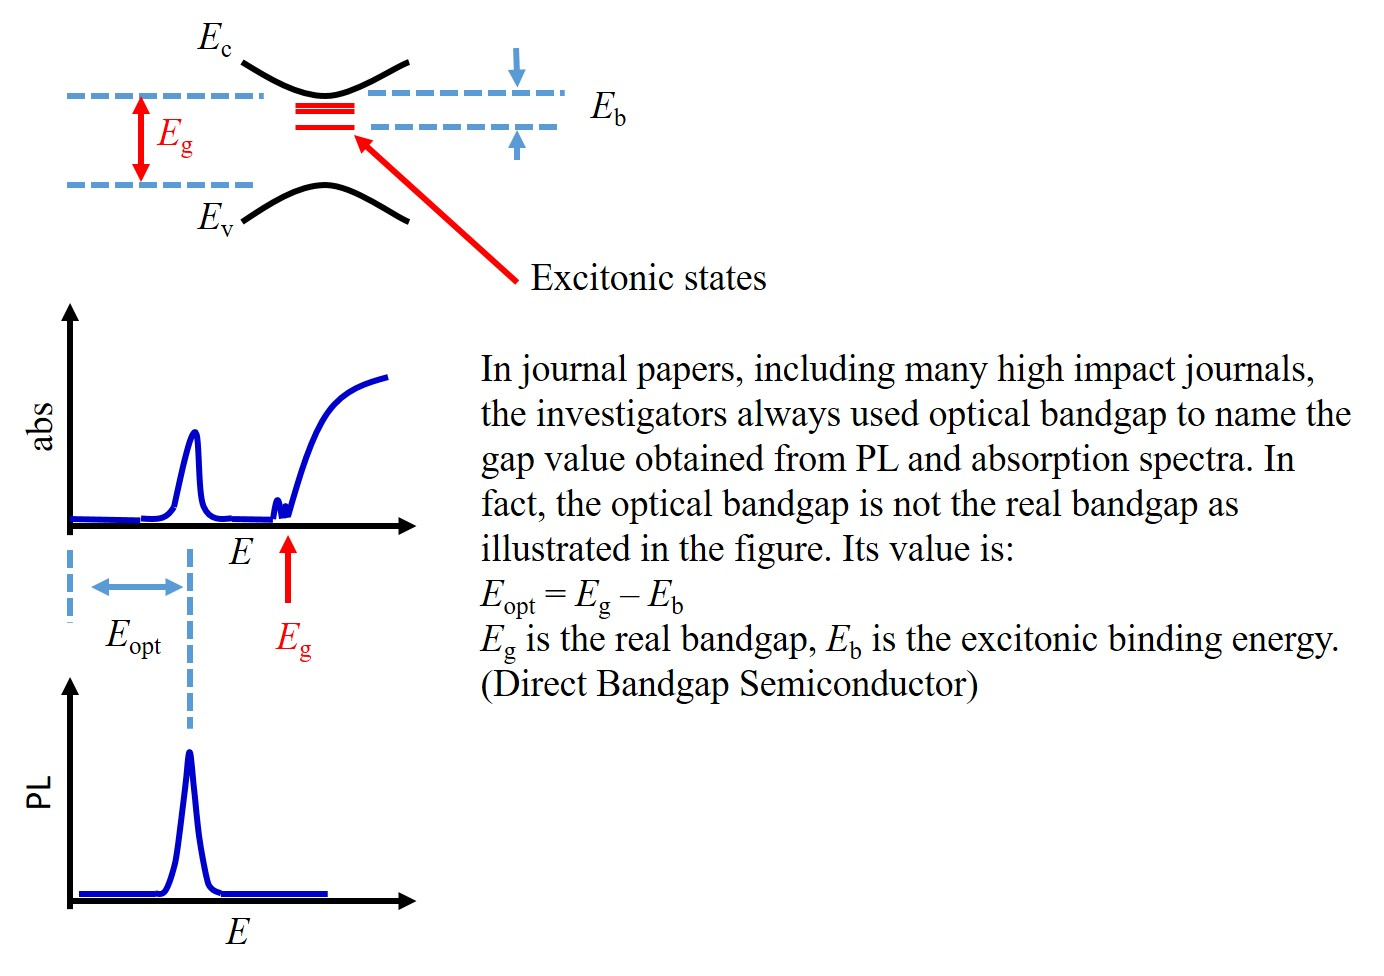
\includegraphics[height=2.4in,width=4.00in,viewport=0 0 670 460,clip]{Figures/Optical_Bandgap.jpg}
\caption{\fontsize{5.2pt}{4.0pt}\selectfont\textrm{Schematic representation of the spectra vs the band gap.}}%
\label{gain-loss_Bandgap}
\end{figure} 
}

\subsection{简单磁性计算}
\frame
{
	\frametitle{\textrm{Heisenberg~}交换模型}
\begin{figure}[h!]
%	\vspace{-0.10in}
\centering
%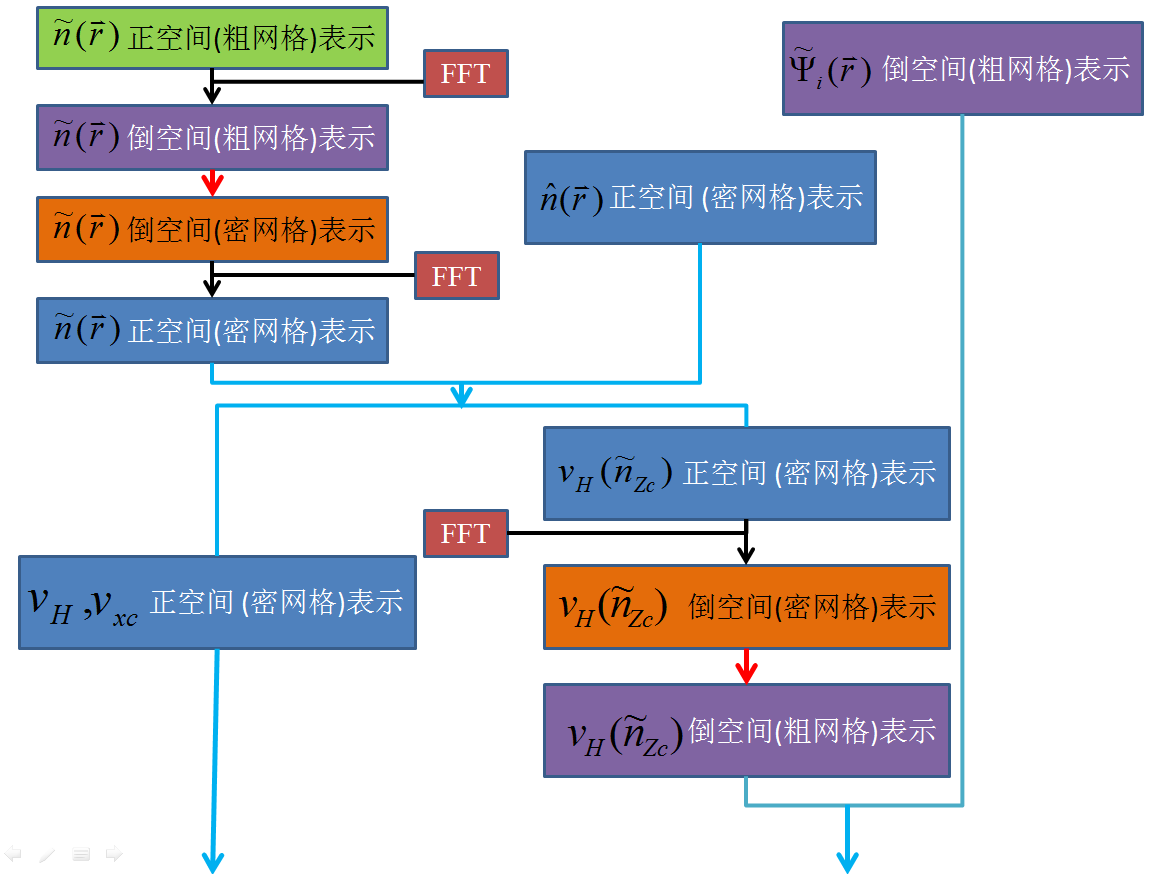
\includegraphics[height=2.7in,width=4.0in,viewport=0 0 1180 875,clip]{Figures/dual_grid.png}
\includegraphics[height=2.0in,width=4.0in,viewport=0 0 580 290,clip]{Figures/Heisenberg_model.jpg}
\caption{\tiny \textrm{The model of Heisenberg-exchange coupling.}}%(与文献\cite{EPJB33-47_2003}图1对比)
\label{Heisenberg_Model}
\end{figure} 
}

\frame
{
	\frametitle{铁磁、反铁磁和亚铁磁}
\begin{figure}[h!]
	\vspace{-0.20in}
\centering
\includegraphics[height=0.95in,width=2.3in,viewport=0 0 350 230,clip]{Figures/Ferromagnetic.jpeg}\\
\includegraphics[height=0.85in,width=2.3in,viewport=0 -13 350 155,clip]{Figures/Antiferromagnetic.png}\\
\includegraphics[height=0.88in,width=2.3in,viewport=0 0 350 225,clip]{Figures/Ferrimagnetic.jpeg}
\caption{\tiny \textrm{The model of Ferromagnetic, Antiferromagnetic and Ferrimagnetic.}}%(与文献\cite{EPJB33-47_2003}图1对比)
\label{Ferrimagneitic_Model}
\end{figure} 
}

\frame
{
	\frametitle{\textrm{Stoner}模型}
	\begin{itemize}
		\item \textrm{Stoner}将金属的磁性考虑为晶格中巡游的$3d$、$4s$\,电子贡献,其相互作用为$I$,\textrm{Fermi}面附近的\textrm{DOS}为$N(E_{\mathrm F})$
\begin{figure}[h!]
\centering
\vspace*{-0.05in}
\includegraphics[height=1.0in,width=1.8in,viewport=0 0 800 380,clip]{Figures/Mag_Metal-T0.png}
\caption{\tiny \textrm{The Stoner model.}}%(与文献\cite{EPJB33-47_2003}图1对比)
\label{Mag_Metal-T0}
\end{figure}
		\item 体系的磁性由转变由\textrm{Fermi}面附近能量变化确定
			\begin{displaymath}
				\Delta E=N(E_{\mathrm F})\big[1-IN(E_{\mathrm F})\big](\delta E)^2
			\end{displaymath}
	\end{itemize}
}

\frame
{
	\frametitle{\textrm{Stoner}模型}
	\begin{itemize}
		\item \textrm{Stoner}模型中参数$I$\,主要反应$3d$电子的紧束缚特征,与晶体结构关系不大
		\item \textrm{Stoner}用于孤立原子体系,参数$I$描述自旋电子的裂分,要求:
			\begin{enumerate}
				\item \textcolor{blue}{对\textrm{LSDA}描述的单行列式态,参数$I$可以精确描述原子态的裂分}
				\item \textcolor{blue}{\textrm{LSDA}中应用\textrm{Stoner}模型,参数$I$\,与\textrm{Hubbard}规则的交换参数$U$一致}
			\end{enumerate}
		\item 参数$U$(或$I$~)、$J$的大小\\
			\begin{enumerate}
				\item \textcolor{red}{\textrm{Hund}规则的交换参数$J$的数量级:~ \textrm{1eV}
				\item \textrm{Hubbard}参数$U$的数量级:~\textrm{10eV}}
			\end{enumerate}
	\end{itemize}
}

\frame
{
	\frametitle{自旋波模型}
	\begin{itemize}
		\item 作为平均场近似,分子场理论成功描述了强磁性物质的自发磁化行为,但在低温和\textrm{Curie}温度附近,理论与实验存在明显偏差
		\item 自旋波理论是从体系\textcolor{red}{整体激发}的角度出发,解释自发磁化的低温行为
			\begin{enumerate}
				\item 0\textrm{K~}下电子自旋有序排列(系统基态)
\begin{figure}[h!]
\centering
\includegraphics[height=0.50in,width=2.45in,viewport=10 10 600 150,clip]{Figures/Mag_spinwave-0.png}
\caption{\tiny \textrm{The ground state $|0\rangle$.}}%(与文献\cite{EPJB33-47_2003}图1对比)
\label{Mag_spinwave-0}
\end{figure}
				\item 温度略有升高时,电子自旋有一个发生翻转
\begin{figure}[h!]
\centering
\includegraphics[height=0.50in,width=2.45in,viewport=10 10 680 150,clip]{Figures/Mag_spinwave-1.png}
\caption{\tiny \textrm{The spin flips at $l$:~ $|l\rangle$.}}%(与文献\cite{EPJB33-47_2003}图1对比)
\label{Mag_spinwave-1}
\end{figure}
			\end{enumerate}
	\end{itemize}
}

\frame
{
	\frametitle{自旋波模型}
	某个格点上出现自旋翻转,\textcolor{blue}{由于相邻格点间存在交换作用,使自旋趋于同向排列}
	\begin{itemize}
		\item \textcolor{red}{翻转的自旋将牵动临近格点自旋,使之趋于翻转}
		\item \textcolor{red}{近邻格点自旋力图驱使翻转的自旋重新翻转过来}
	\end{itemize}
	自旋的翻转不会停留在一个格点,而是以波的形式向周围传播:\\
	\textcolor{blue}{这种自旋翻转在晶体中的传播称为}\textcolor{red}{自旋波(又称磁激子)}
\begin{figure}[h!]
\centering
\includegraphics[height=1.15in,width=3.45in,viewport=0 0 830 300,clip]{Figures/Mag_spinwave-2.png}
\caption{\tiny \textrm{The schematic spin-wave.}}%(与文献\cite{EPJB33-47_2003}图1对比)
\label{Mag_spinwave-2}
\end{figure}
}

\frame
{
	\frametitle{非共线磁矩}
	\begin{itemize}
		\item 真实的物理体系中总会出现非共线的磁结构:\\\textcolor{blue}{特别是在铁磁/非磁金属界面上,铁磁性原子磁矩有可能形成非共线排列}
		\item 非共线体系中出现的新现象:\textcolor{blue}{电流诱导的自旋转矩}\\
			\textcolor{red}{非共线的原子磁矩与电子的自旋之间能够通过交换作用,进而引起电子在输运过程中发生自旋翻转,使得自旋向上和自旋向下的输运通道发生了混合}%,并且处在超导态的非磁金属还能够在铁磁体一侧诱导出长程的自旋三重态配对超导性}
		\item 由于非共线磁结构的引入使得问题变得复杂,目前的实验和理论还并不完备
	\end{itemize}
\begin{figure}[h!]
\centering
\vspace*{-0.10in}
\includegraphics[height=1.05in,width=2.40in,viewport=10 10 840 370,clip]{Figures/Magnet_spinal_wave.png}
\caption{\tiny \textrm{The spiral magnetic structure.}}%(与文献\cite{EPJB33-47_2003}图1对比)
\label{Mag_spinal-wave}
\end{figure}
}

\section{遗传算法与结构预测}
\frame
{
	\frametitle{深度神经网络基础}
	\begin{itemize}
		\item 感知机(\textrm{Perceptron Learning Algorithm, PLA}):~最早的监督式训练算法,是神经网络构建的基础
\begin{figure}[h!]
\vspace*{-0.08in}
\centering
\includegraphics[height=0.50in]{Figures/DNN_PLA.png}
\caption{\tiny \textrm{Perceptron Learning Algorithm.}}%(与文献\cite{EPJB33-47_2003}图1对比)
\label{Fig:PLA}
\end{figure}
输出与输入之间将学习到一个线性关系,可有中间输出结果
\begin{displaymath}
	z=\sum_{i=1}^mw_ix_i+b
\end{displaymath}
中间结果连接一个神经元激活函数
\begin{displaymath}
	\mathrm{sign}(z)=\left\{
		\begin{aligned}
			-1\qquad &z<0\\
			1 \qquad &z\geqslant 0
		\end{aligned}\right.
\end{displaymath}
	\end{itemize}
}

\frame
{
	\frametitle{深度神经网络基础}
\begin{figure}[h!]
\vspace*{-0.08in}
\centering
\includegraphics[width=2.5in]{Figures/NN_PLA_example.png}
%\caption{\tiny \textrm{Perceptron Learning Algorithm.}}%(与文献\cite{EPJB33-47_2003}图1对比)
\label{Fig:PLA}
\end{figure}
在本例中,每一个输入数据都可以表示为一个向量$x = (x_1, x_2)$ ,而函数则是要实现“如果线以下,输出0;线以上,输出1”
}

\frame
{
	\frametitle{深度神经网络基础}
感知机模型只能用于二元分类,无法学习较为复杂的非线性模型,神经网络在感知机模型基础上作了扩展
\vskip 10pt
	\begin{itemize}
		\item 加入隐藏层(\textrm{hide layer}):~隐藏层可以有很多层,增强模型的表达能力
		\item 输出层的神经元可以有不止一个输出
		\item 对激活函数作扩展,如\textrm{Sigmoid}函数
			\begin{displaymath}
				f(z)=\dfrac1{1+\mathrm{e}^{-z}}
			\end{displaymath}
			其他的激活函数还有\textrm{tanx}、\textrm{softmax}和\textrm{ReLU}等
	\end{itemize}
}

\frame
{
	\frametitle{深度神经网络}
当前的深度神经网络~\textrm{(Deep Learning Neural Network)}~可以包含上百层神经元,通常有上万个参数,再加上超参数,实际的参数空间几乎是无限大的。如何从海量潜在的可能参数中做选择极具挑战性。
\begin{figure}[h!]
\vspace*{-0.08in}
\centering
\includegraphics[height=1.75in,width=3.75in]{Figures/ANN_Algorithm.png}
\caption{\tiny \textrm{Deep Learning Neural Network.}}%(与文献\cite{EPJB33-47_2003}图1对比)
\label{Fig:Deep-Learning-NN}
\end{figure}
}

\frame
{
	\frametitle{深度神经网络的前馈算法}
	以三层深度神经网络为例,说明深度神经网络的前馈算法
\begin{figure}[h!]
\vspace*{-0.08in}
\centering
\includegraphics[width=3.0in]{Figures/DNN_front_pro.jpg}
%\caption{\tiny \textrm{Perceptron Learning Algorithm.}}%(与文献\cite{EPJB33-47_2003}图1对比)
\label{Fig:PLA}
\end{figure}
}

\frame
{
	\frametitle{遗传算法的基本原理}
	遗传算法\textrm{(Genetic Algorithm, GA)}是模拟生物进化论的自然选择和遗传学机理的计算模型,\textcolor{blue}{通过模拟自然进化过程搜索最优解}
	\begin{enumerate}
%		\item 优化问题可能潜在的解集构成一个种群(\textrm{population}),该种群由经过基因(\textrm{gene})编码的一定数目的个体(\textrm{individual})组成,每个个体是染色体(\textrm{chromosome})带有特征的实体
		\item 优化问题可能潜在的解集构成一个种群,该种群由经过基因编码的一定数目的个体组成,每个个体是带有一定的优化特征
%		\item 种群产生之后,借助于自然遗传学的遗传算子(\textrm{genetic operators})进行组合交叉(\textrm{crossover})和变异(\textrm{mutation}),产生新一代个体
		\item 种群产生之后,借助于自然遗传学的遗传算子进行组合交叉(\textrm{crossover})和变异(\textrm{mutation}),产生新一代个体
\begin{figure}[h!]
\vspace*{-0.10in}
\centering
\includegraphics[width=2.5in]{Figures/Genetic_Algorithm_basic.png}
%\caption{\tiny \textrm{Perceptron Learning Algorithm.}}%(与文献\cite{EPJB33-47_2003}图1对比)
\label{Fig:PLA}
\end{figure}
%		\item 按照适者生存和优胜劣汰的原理,在每一代,根据问题域中个体的适应度(\textrm{fitness}),选择(\textrm{selection})合适的个体,构成代表新的解集的种群
\vspace*{-0.10in}
		\item 按照适者生存和优胜劣汰的原理,在每一代,根据问题域中个体的适应度,选择合适的个体,构成代表新的解集的种群
%		\item 逐代(\textrm{generation})演化后,产生出越来越好的近似解(优化目标)
		\item 逐代演化后,产生出越来越好的近似解(优化目标)
	\end{enumerate}
}

\frame
{
	\frametitle{深度神经网络与遗传算法}
	\textcolor{blue}{深度神经网络类似问题的解决方案:~遗传算法}
\begin{minipage}[b]{0.49\textwidth}
\includegraphics[height=0.4in,width=2.08in,viewport=0 110 1280 350,clip]{Figures/Genetic_Algorithm-2.png}\\
\centering{\includegraphics[height=1.0in,width=1.08in,viewport=140 50 820 650,clip]{Figures/Genetic_Algorithm-1.png}}\\
\vskip 0.02pt
\includegraphics[height=0.7in,width=2.05in]{Figures/Genetic_Algorithm-3.png}\\
\centering{\textcolor{red}{\textrm{\tiny GACNN:~利用遗传算法训练深度卷积神经网络}}}
\end{minipage}
\hfill
\begin{minipage}[b]{0.49\textwidth}
\includegraphics[height=1.2in,width=1.9in]{Figures/Genetic_Algorithm-5.png}\\
\vskip 0.5pt
\includegraphics[height=0.55in,width=1.95in]{Figures/Genetic_Algorithm-4.png}\\
\centering{\textcolor{red}{\textrm{\tiny 多智能体强化学习:~神经网络}}}
\end{minipage}
}

\frame
{
	\frametitle{晶体结构优化的复杂性}
	\begin{itemize}
		\item \textcolor{blue}{晶体结构预测与搜索中也遇到类似问题}\\
		在已知元素种类的条件下,有可能预测或搜索材料晶体的结构;~但是材料的等能面存在无数个局域极小点,因而可能的晶体结构也是无限多的\\
		这使得晶体结构的预测与搜索极其困难
\begin{figure}[h!]
\centering
\includegraphics[height=1.3in,width=1.3in]{Figures/Struct-predict-3.png}
\hskip 1.0pt
\includegraphics[height=1.1in,width=2.25in]{Figures/Total_energy_opt.png}
\caption{\tiny \textrm{The structure of Perovskite and schematic for the energy minimum searching.}}%(与文献\cite{EPJB33-47_2003}图1对比)
\label{Fig:Structure-optimized}
\end{figure}
	\end{itemize}
}

\frame
{
	\frametitle{晶体结构优化问题的解决}
	\textcolor{blue}{解决方案:~遗传算法、粒子群方法等}
\begin{figure}[h!]
\centering
\includegraphics[height=1.0in,width=1.7in]{Figures/Struct-predict-1.png}
\includegraphics[height=1.0in,width=2.2in]{Figures/Struct-predict-2.png}
\vskip 3.0pt
\includegraphics[height=0.7in,width=2.2in]{Figures/Logo_USPEX.png}
\hskip 1.0pt
\includegraphics[height=0.8in,width=1.8in]{Figures/Logo_Calypso.png}
%\caption{\tiny \textrm{The structure of Perovskite and schematic for the energy minimum searching.}}%(与文献\cite{EPJB33-47_2003}图1对比)
\label{Fig:Structure-optimized-2}
\end{figure}
}

%-----------------------------------------------------------------------------------------------------------------------------------------------------------------------%
\section{复杂磁性结构}
\frame
{
	\frametitle{磁随机存储器\textrm{(MRAM)}}
磁性材料的核心问题:材料自旋磁结构的构筑、调控与设计
\begin{figure}[h!]
%\vspace*{-0.08in}
\centering
\includegraphics[height=1.85in,width=4.05in]{Figures/MRAM-Devices.png}
%\caption{\tiny \textrm{Simple Magnetic structure:~Ferromagnetism, Anti-Ferromagnetism, Ferrimagnetism}}%(与文献\cite{EPJB33-47_2003}图1对比)
\label{Fig:MRAM-Devices}
\end{figure}
}

\frame
{
	\frametitle{磁随机存储器\textrm{(MRAM)}}
	\begin{itemize}
		\item {\tiny \textrm{日本东北大学的科研团队成功开发出存储密度达128\textrm{Mb}的\textrm{STT-MRAM},写入速度达14\textrm{ns},可作为物联网和人工智能中用到的缓存使用}}
\begin{figure}[h!]
\vspace*{-0.08in}
\centering
\includegraphics[height=1.00in,width=1.65in]{Figures/Si-crystal-Surface.png}
%\caption%(与文献\cite{EPJB33-47_2003}图1对比)
\label{Fig:Si-crystal-surface}
\end{figure}
\item {\tiny \textrm{韩国\textrm{Samsung}公司宣布已在一条基于28\textrm{nm~FD-SOI}工艺的生产线上,开始大规模生产和商业运输嵌入式\textrm{MRAM(eMRAM)}解决方案}}
\begin{figure}[h!]
\vspace*{-0.08in}
\centering
\includegraphics[height=1.00in,width=1.60in]{Figures/Samsung-cell.png}
%\caption%(与文献\cite{EPJB33-47_2003}图1对比)
\label{Fig:Samsung-cell}
\end{figure}
	\end{itemize}
}

\frame
{
	\frametitle{\textcolor{red}{开发\textrm{MRAM}技术瓶颈问题}}
	\begin{itemize}
		\item 如何构建一套具有范式意义的技术方法,使得我们能够\textcolor{red}{快速、精准地预测各类磁性材料的磁结构及磁参数}\\
			对加速开发\textrm{MRAM}具有至关重要的作用,目前属于国际空白
\begin{figure}[h!]
\vspace*{-0.04in}
\centering
\includegraphics[height=2.15in,width=3.25in]{Figures/Magnet-skyrmion.png}
%\caption{\tiny \textrm{}}%(与文献\cite{EPJB33-47_2003}图1对比)
\label{Fig:Magnet-skyrmion}
\end{figure}
	\end{itemize}
}

\frame
{
	\frametitle{简单磁结构~\textrm{.VS.}~复杂磁结构}
\begin{figure}[h!]
\vspace*{-0.08in}
\centering
\includegraphics[height=1.05in,width=0.75in]{Figures/Magnet-simple.png}
\caption{\tiny \textrm{Simple Magnetic structure:~Ferromagnetism, Anti-Ferromagnetism, Ferrimagnetism}}%(与文献\cite{EPJB33-47_2003}图1对比)
\label{Fig:Simple-Magnet}
\end{figure}
\begin{figure}[h!]
\vspace*{-0.08in}
\centering
\includegraphics[height=1.05in,width=2.35in]{Figures/Magnet-complex-compound.png}
\hskip 0.5pt
\includegraphics[height=1.05in,width=1.35in]{Figures/Magnet-complex.png}
\caption{\tiny \textrm{Complex Magnetic structure:~Spiral magnet, All-in-all-out, 3k-ordered}}%(与文献\cite{EPJB33-47_2003}图1对比)
\label{Fig:Simple-Magnet}
\end{figure}
}

\frame
{
	\frametitle{复杂磁结构的两大起源}
	\begin{itemize}
		\item 强磁阻挫:~\textrm{Kagome}晶格
\begin{figure}[h!]
\vspace*{-0.08in}
\centering
\includegraphics[height=0.7in,width=1.5in]{Figures/Magnet-Kagome-lattice.png}
\caption{\tiny \textrm{The Kagome lattice}}%(与文献\cite{EPJB33-47_2003}图1对比)
\label{Fig:Magnet-Kamoge}
\end{figure}
		\item 强自旋-轨道耦合:~稀土、锕系元素,核材料
\begin{figure}[h!]
\vspace*{-0.08in}
\centering
\includegraphics[height=0.85in,width=1.4in]{Figures/Magnet-Strong-SOC.png}
\includegraphics[height=0.85in,width=1.4in]{Figures/Nuclear-Power.png}
\caption{\tiny \textrm{Strong spin-orbit coupling and nuclear materials.}}%(与文献\cite{EPJB33-47_2003}图1对比)
\label{Fig:Magnet-SOC}
\end{figure}
	\end{itemize}
}

\frame
{
	\frametitle{确定磁结构的方法和困难}
	\begin{itemize}
                \setlength{\itemsep}{5pt}
		\item \textcolor{blue}{确定磁结构的常用方法}
			\begin{enumerate}
                                \setlength{\itemsep}{3pt}
				\item 实验方法:~中子散射
				\item 理论方法:~人工猜测-计算验证方法
				\item 理论方法:~拟合磁自由度\textrm{Hamiltonian}-模拟退火
			\end{enumerate}
		\item \textcolor{blue}{复杂磁有序结构测定的困难}
			\begin{enumerate}
                                \setlength{\itemsep}{3pt}
				\item 中子散射:~某些实验材料质量欠佳、极端条件
				\item 人工猜想-计算验证方法:~效率低下,不适合复杂材料
				\item \textrm{Hamiltonian}-模拟退火:~\textrm{Hamiltonian}拟合困难,精度无法保证
			\end{enumerate}
			\textcolor{red}{本质的困难}:~海量潜在的可能结构导致常用方法失效
	\end{itemize}
}

\frame
{
	\frametitle{磁结构遗传算法预测软件\textrm{MagGene}}
鉴于遗传算法在深度学习和晶体结构预测中的成功应用,这种方法在磁结构预测中也大有用武之地。\textrm{MagGene}就是整合遗传算法和常用的第一性原理计算软件预测材料磁结构新型软件。
\begin{figure}[h!]
\centering
\includegraphics[height=2.2in,width=2.2in]{Figures/MagGene-Flow.png}
\caption{\tiny \textrm{The flow of MagGene.}}%(与文献\cite{EPJB33-47_2003}图1对比)
\label{Fig:MagGene-Flow}
\end{figure}
}

\appendix
\section{高通量材料计算平台开发现状}     %Bookmark
\frame
{
	\frametitle{国内已有的计算平台:~\textrm{MatCloud}}
\begin{figure}[h!]:
\centering
\includegraphics[height=1.57in,width=4.95in,viewport=0 0 1800 550,clip]{Figures/Matcloud-login.png}
\caption{\fontsize{7.2pt}{4.2pt}\selectfont{中科院计算机网络信息中心~杨小渝团队开发}\upcite{CMS146-319_2018,url_Matcloud}}%
\label{Auto_Flow_Platform-2}
\end{figure}
}

\frame
{
	\frametitle{国外已有的计算平台}
\begin{figure}[h!]
\centering
\vspace{-15.5pt}
\subfigure[\fontsize{7.5pt}{6.2pt}\selectfont{\textrm{Auto-FLOW (AFLOW)}\upcite{CMS58-227_2012}}]{
\label{AFLOW_data_flow}
\includegraphics[height=1.2in,width=1.6in,viewport=0 0 720 660,clip]{Figures/AFLOW_database.png}}
\subfigure[\fontsize{7.5pt}{6.2pt}\selectfont{\textrm{Material Project (MP)}\upcite{CMS97-209_2015}}]{
\label{MP_commp_infrastructure}
\includegraphics[height=1.2in,width=1.7in,viewport=0 0 670 530,clip]{Figures/MP_comp_infrastructure.png}}
\subfigure[\fontsize{3.5pt}{3.2pt}\selectfont{\textrm{Quantum Materials Informatics Project (QMIP)}\upcite{url_QMIP}}]{
\label{QMIP_Shame}
\includegraphics[height=1.2in,width=1.7in,viewport=0 0 670 420,clip]{Figures/QMIP_shame.png}}
\subfigure[\fontsize{6.5pt}{5.2pt}\selectfont{\textrm{Clean Energy Project (CEP)}\upcite{JPCL2-2241_2011}}]{
\label{CEP_structure_flow}
\includegraphics[height=1.2in,width=1.6in,viewport=0 0 1020 730,clip]{Figures/CEP_structure_flow.png}}
%\caption{}%
\label{Auto_Flow_Platform-1}
\end{figure}
}

\frame
{
	\frametitle{\textrm{ASE}:~接口丰富的适应性计算平台}
\begin{figure}[h!]
\centering
\vspace*{-0.2in}
\includegraphics[height=2.1in,width=3.2in,viewport=0 0 1208 830,clip]{Figures/ASE_Python_lib.png}
\caption{\fontsize{7.2pt}{4.2pt}\selectfont{\textrm{ASE:~a Python library for working with atoms.}}}%
\label{Logo_ASE_lib}
\end{figure} 
}

\frame
{
	\frametitle{\textrm{Atomly}:~物理所的无机晶体材料计算数据库}
\begin{figure}[h!]
\centering
\vspace*{-0.2in}
\includegraphics[height=2.1in,width=4.1in,viewport=5 0 1608 830,clip]{Figures/Atomly.png}
\caption{\fontsize{7.2pt}{4.2pt}\selectfont{\textrm{Atomly:~中科院物理所~刘淼等老师开发,数据库包含了17万\!$^+$\!无机晶体材料第一性原理计算结果\textrm{(包含电子结构信息:~DOS~+~energy~bands)}.}}}%
\label{Logo_Atomly_lib}
\end{figure} 
}

\frame
{
	\frametitle{\textrm{计算平台的功能和总体架构}}
\begin{figure}[h!]
\centering
\vspace*{-0.35in}
\includegraphics[height=2.6in,width=4.05in,viewport=0 0 670 460,clip]{Figures/Parallel_computation.png}
%\includegraphics[height=1.6in,width=2.4in,viewport=0 0 1038 730,clip]{Figures/Auto_Flow.png}
\caption{\fontsize{7.2pt}{4.2pt}\selectfont{\textrm{The schematic framework and platform of all those project.}}}%
\label{Auto_Flow}
\end{figure} 
}

\frame
{
	\frametitle{现有高通量计算平台概览}
\begin{table}[!h]
\tabcolsep 0pt \vspace*{-12pt}
%\caption{}
\label{Table-Cost}
\begin{minipage}{0.85\textwidth}
%\begin{center}
\centering
\def\temptablewidth{1.1\textwidth}
\renewcommand\arraystretch{0.8} %表格宽度控制(普通表格宽度的两倍)
\rule{\temptablewidth}{1pt}
\begin{tabular*} {\temptablewidth}{@{\extracolsep{\fill}}c@{\extracolsep{\fill}}c@{\extracolsep{\fill}}c@{\extracolsep{\fill}}c@{\extracolsep{\fill}}c@{\extracolsep{\fill}}c@{\extracolsep{\fill}}c}
%-------------------------------------------------------------------------------------------------------------------------
	&\multirow{2}{*}{\fontsize{7.2pt}{5.2pt}\selectfont{编程语言}}	&\fontsize{7.2pt}{5.2pt}\selectfont{建模} &\multicolumn{2}{|c|}{\fontsize{6.2pt}{5.2pt}\selectfont{任务提交与管理}} &\multirow{2}{*}{\fontsize{7.2pt}{5.2pt}\selectfont{后处理}} &\multirow{2}{*}{\fontsize{6.2pt}{5.2pt}\selectfont{数据组织管理}} \\\cline{4-5}
	&	&\fontsize{7.2pt}{5.2pt}\selectfont{功能} &\multicolumn{1}{|l}{\fontsize{7.2pt}{5.2pt}\selectfont{软件接口}} &\multicolumn{1}{r|}{\fontsize{7.2pt}{5.2pt}\selectfont{运行容错}} & & \\\hline
	\fontsize{7.2pt}{5.2pt}\selectfont{{AFLOW}} &\fontsize{7.2pt}{5.2pt}\selectfont{C++} &\checkmark &$\triangle$ &\FiveStarOpen &\FiveStarOpen &\fontsize{7.2pt}{5.2pt}\selectfont{{Django}} \\
	\fontsize{7.2pt}{5.2pt}\selectfont{{MP}} &\fontsize{7.2pt}{5.2pt}\selectfont{Python} &\checkmark &\checkmark &\FiveStarOpen &\FiveStarOpen &\fontsize{7.2pt}{5.2pt}\selectfont{{MongoDB}} \\
	\multirow{2}{*}{\fontsize{7.2pt}{5.2pt}\selectfont{{QMIP}}} &\fontsize{7.2pt}{5.2pt}\selectfont{JavaScript/SVG} &\multirow{2}{*}{\checkmark} &\multirow{2}{*}{\checkmark} &\multirow{2}{*}{--} &\multirow{2}{*}{\checkmark} &\multirow{2}{*}{--} \\
	&\fontsize{7.2pt}{5.2pt}\selectfont{+html/Python} & & & & & \\
	\fontsize{7.2pt}{5.2pt}\selectfont{{CEP}} &\fontsize{7.2pt}{5.2pt}\selectfont{Python} &\checkmark &\checkmark &-- &\checkmark &\fontsize{7.2pt}{5.2pt}\selectfont{{Django/MySQL}} \\
	\fontsize{7.2pt}{5.2pt}\selectfont{{ASE}} &\fontsize{7.2pt}{5.2pt}\selectfont{Python} &\FiveStarOpen &\FiveStarOpen &-- &$\triangle$ &-- \\
	\multirow{2}{*}{\fontsize{7.2pt}{5.2pt}\selectfont{{MatCloud}}} &\fontsize{7.2pt}{5.2pt}\selectfont{JavaScript} &\multirow{2}{*}{\checkmark} &\multirow{2}{*}{$\triangle$} &\multirow{2}{*}{\checkmark} &\multirow{2}{*}{\checkmark} &\multirow{2}{*}{\fontsize{7.2pt}{5.2pt}\selectfont{{MongoDB}}} \\
	&\fontsize{7.2pt}{5.2pt}\selectfont{+.NETCore} & & & & &
\end{tabular*}
\rule{\temptablewidth}{1pt}
\end{minipage}
%\vskip -15pt
\fontsize{7.2pt}{5.2pt}\selectfont{
\begin{description}
	\item[\FiveStarOpen]~该功能较突出
	\item[\checkmark]~该功能基本满足需求
	\item[$\triangle$]~该功能存在不足
\end{description}}
%\end{center}
\end{table}
\fontsize{8.2pt}{6.2pt}\selectfont{
	\textrm{Lin L. \textit{Materials databases infrastructure constructed by first principles calculations:~a review.} \textbf{Mater. Perform. Character.}, 2015, 4(1):148.}}
}

\subsection{\rm{MP}与\rm{ASE}}     %Bookmark
\frame
{
	\frametitle{\textrm{MP}自动流程的设计与开发}
	\begin{itemize}
		\item \textcolor{red}{设计目标}:~围绕\textrm{VASP~}作业高通量并发提交与过程监控
		\item \textcolor{red}{设计方案}:~开发针对不同计算场景的功能模块
			\begin{enumerate}
    \setlength{\itemsep}{15pt}
				\item \textcolor{blue}{\textbf{Pymatgen}}\\
					\textcolor{magenta}{前处理}:~计算模型的分析与预处理\\
					\textcolor{magenta}{后处理}:~计算结果的可视化
				\item \textcolor{blue}{\textbf{FireWorks}}\\
\textcolor{magenta}{计算流程设计与管理}:~数据库支持的计算流程管理
				\item \textcolor{blue}{\textbf{Custodian}}\\
\textcolor{magenta}{计算流程容错与应对}:~提供计算过程错误判断接口,由用户提供解决策略和针对性设计
			\end{enumerate}
	\end{itemize}
		%\item 计算过程的控制方式
}

\frame
{
	\frametitle{\textrm{Pymatgen}的模块结构}
\begin{figure}[h!]
\centering
\vspace*{-0.1in}
\includegraphics[height=2.3in]{Figures/MP_library.png}
\caption{\fontsize{7.2pt}{4.2pt}\selectfont{\textrm{Overview of a typical workflow for pymatgen.}}}%
\label{Pymatgen_Lib}
\end{figure} 
}

\frame
{
	\frametitle{\textrm{Pymatgen}可展示的材料物性}
\begin{figure}[h!]
\centering
\vspace*{-0.1in}
\includegraphics[height=2.3in]{Figures/MP_vision.png}
\caption{\fontsize{5.2pt}{4.2pt}\selectfont{\textrm{Top left: Phase; Top right: Pourbaix diagram from the Materials API. \\Bottom left: Calculated bandstructure plot using pymatgen’s parsing and plotting utilities. Bottom right: Arrhenius plot using pymatgen’s Diffusion~Analyzer.}}}%
\label{Pymatgen_vision}
\end{figure} 
}

\frame
{
	\frametitle{\textrm{FireWorks}的模块结构}
\textrm{FireWorks}发布的工作流成由三层嵌套结构组成:
\fontsize{8.2pt}{6.2pt}\selectfont{
\begin{itemize}
	\item \textrm{Firetask}:~基本执行单元,是执行计算的最基本脚本命令或\textrm{Python}命令。
	\item \textrm{Firework}:~组织基本执行单元构成任务单元组,并指定各基本执行单元所需的参数。
	\item \textrm{Workflow}:~彼此相关联的任务单元组构成完整的工作流程:\\
		\textrm{FireWork}之间的数据传递、任务执行序列等由\textrm{FWAction}完成。
\end{itemize}}
\begin{figure}[h!]
\centering
\vspace*{-0.1in}
\includegraphics[height=1.5in]{Figures/MP_fireworks.png}
\hskip 1pt
\includegraphics[height=1.5in]{Figures/MP_multiple_fw.png}
\caption{\fontsize{7.2pt}{4.2pt}\selectfont{\textrm{The basic infrastructure of FireWorks.}}}%
\label{FireWorks_FW}
\end{figure} 
}

\frame
{
	\frametitle{\textrm{atomate}:~计算流程控制示范}
%		\textcolor{purple}{\textrm{Atomate}}:~:~适合一定复杂程度的\textrm{~VASP~}计算
\begin{figure}[h!]
\centering
\vspace*{-0.19in}
\includegraphics[height=1.4in,width=2.2in,viewport=0 0 820 630,clip]{Figures/Atomate_comp.png}
\vskip 1pt
\includegraphics[height=1.5in]{Figures/bandstructure_wf.png}
%\caption{\fontsize{7.2pt}{4.2pt}\selectfont{\textrm{The integrated calculator in ASE (Atomic Simulation Environment).}}}%
\label{Logo_QM-MM}
\end{figure} 
}

\frame
{
	\frametitle{\textrm{ASE}自动流程的设计与管理}
		\textcolor{purple}{\textrm{ASE}}:~模块加载式计算流程控制,更符合复杂多尺度计算场景
		\begin{itemize}
			\item \textcolor{magenta}{灵活的建模功能}
				\begin{enumerate}
    \setlength{\itemsep}{10pt}
					\item 简单堆积:~原子直接组成分子
					\item 理想周期体系(包括一维、二维、三维)
					\item 表面和表面吸附,可指定吸附位
				\end{enumerate}
			\item \textcolor{magenta}{丰富的软件接口}\\
				提供了包括绝大部分第一原理和分子动力学计算软件接口,方便组合实现多尺度计算
			\item \textcolor{magenta}{不依赖软件的优化与动力学模拟}\\
				适合复杂材料物性模拟的优化和多种动力学过程模拟
			\item \textcolor{magenta}{多样化的数据库类型}
		\end{itemize} 
}

\frame
{
\frametitle{\textrm{ASE}特色:~材料结构生成模块}
\begin{figure}[h!]
\centering
\vspace*{-0.15in}
\includegraphics[height=1.2in,width=1.7in,viewport=0 0 820 530,clip]{Figures/ASE_atoms_module.png}
\includegraphics[height=2.9in,width=2.2in,viewport=0 0 970 1200,clip]{Figures/ASE_atoms_module-examples.png}
%\caption{\fontsize{7.2pt}{4.2pt}\selectfont{\textrm{The integrated calculator in ASE (Atomic Simulation Environment).}}}%
\label{Logo_atoms-module}
\end{figure} 
}

\frame
{
\frametitle{\textrm{ASE}特色:~软件接口丰富}
\textcolor{purple}{\textrm{ASE}}:~\textrm{Calculator}模块提供的可选的软件接口
\begin{figure}[h!]
\centering
\vspace*{-0.05in}
%\includegraphics[height=1.0in,width=1.4in,viewport=0 0 638 530,clip]{Figures/ASE_calculator.png}
\includegraphics[height=2.0in,width=3.2in,viewport=0 0 940 600,clip]{Figures/ASE_calculator-new.png}
\caption{\fontsize{7.2pt}{4.2pt}\selectfont{\textrm{The integrated calculator in ASE.}}}%
\label{ASE_Calculator}
\end{figure} 
}

\frame
{
\frametitle{\textrm{ASE}特色:~提供多种优化算法模块和数据库}
\begin{figure}[h!]
\centering
\vspace*{-0.18in}
\includegraphics[height=1.3in,width=2.5in,viewport=0 0 838 500,clip]{Figures/ASE_opt_modules.png}
\vskip 1pt
\includegraphics[height=1.7in,width=2.5in,viewport=0 0 938 630,clip]{Figures/ASE_database.png}
\label{ASE_opt-database}
\end{figure} 
}

\frame
{
	\frametitle{}
\begin{figure}[h!]
\centering
\vspace{-5.5pt}
\includegraphics[height=0.65\textwidth]{Figures/Quote-Huang_Kun.jpg}
\caption{\fontsize{6.2pt}{5.2pt}\selectfont{黄昆~教授的治学名言}}
\label{Quote-Huang_Kun}
\end{figure}
}
%------------------------------------------------------------------------Reference----------------------------------------------------------------------------------------------
		\frame[allowframebreaks]
{
\frametitle{主要参考文献}
\begin{thebibliography}{99}
{\tiny
	\bibitem{VASP_manual}\textrm{G. Kresse and M. Marsman and J. Furthm\"uller, \textit{Vienna Ab-initio Simulation Package~\textrm{(VASP)} the Guide}. Computational Materials Physics, Faculty of Physics, Universit\"at Wien, Austria (2016)}
	\bibitem{WIEN2k_UG}\textrm{P. Blaha, K. Schwarz, G. Madsen, D. Kvasnicka and J. Luitz. \textit{User's Guide of WIEN2K, An Augmented Plane Wave Plus Local Orbitals Program for Calculating Crystal Properties}. Vienna University of Technology, Inst. of Physical and Theoretical Chemistry, Vienna, Austria (2012)}
	\bibitem{CMS146-319_2018}\textrm{X. Yang, Z. Wang, X. Zhao and H. Liu \textit{Comp. Mater. Sci.}, \textbf{146} (2018), 319}
	\bibitem{url_Matcloud}\textrm{\url{http://matcloud.cnic.cn}}
	\bibitem{CMS58-227_2012}\textrm{S. Curtarolo, W. Setyawan, S. Wang, J. Xue, K. Yang, R. H. Taylor, L. J. Nelson, G. L. Hart, S. Sanvito, M. Buongiorno-Nardelli, N. Mingo and O. Levy \textit{Comp. Mater. Sci.}, \textbf{58} (2012), 227}
	\bibitem{CMS97-209_2015}\textrm{S. P. Ong, S. Cholia, A. Jain, M. Brafman, D. Gunter, G. Ceder and K. A. Persson. \textit{Comp. Mater. Sci.}, \textbf{97} (2015), 209}
	\bibitem{url_QMIP}\textrm{\url{http://www.qmip.org/qmip.org/Welcome.html}}
	\bibitem{JPCL2-2241_2011}\textrm{J. Hachmann, R. Olivares-Amaya, S. Atahan-Evrenk, C. Amador-Bedolla, R. S. S$\acute{a}$nchez-Carrera, A. Gold-Parker, L. Vogt, A. M. Brockway and A. Aspuru-Guzik \textit{J. Phys. Chem. Lett.}, \textbf{2} (2011), 2241}
%	\bibitem{url_Mater_Genome}\textrm{\url{https://www.whitehouse.gov/sites/default/files/microsites/ostp/materials_genome_initiative-final.pdf}}
%	\bibitem{CMS49-299_2010}\textrm{W. Setyawan and S. Curtarolo \textit{Comp. Mater. Sci.}, \textbf{49} (2010), 299}
%	\bibitem{CMS50-2295_2011}\textrm{A. Jain, G. Hautier, C. J. Moore, S. P. Ong, C. C. Fischer, T. M. Kristin, K. A. Persson and G. Ceder \textit{Comp. Mater. Sci.}, \textbf{50} (2011), 2295}
%	\bibitem{unpublished}\textrm{D. Gunter, S. Cholia, A. Jain, M. Kocher, K. Persson, L. Ramakrishnan, S. P. Ong and G. Ceder. \textit{Community Accessible Datastore of High-Throughput Calculations: Experiences from the Materials Project} (unpublished)}
	\bibitem{MPC4-148_2015}\textrm{L. Lin \textit{Mater. Perform. Character.}, \textbf{4} (2015), 148}
}
\end{thebibliography}
%\nocite*{}
}
